\documentclass[11pt,a4paper]{article}

% ── Fonts & Encoding ────────────────────────────────────────────────────────
\usepackage[T1]{fontenc}
\usepackage[utf8]{inputenc}
\usepackage{helvet}          % Arial substitute (Helvetica)
\renewcommand{\familydefault}{\sfdefault}

% ── Page Layout ─────────────────────────────────────────────────────────────
\usepackage[a4paper, margin=2.5cm]{geometry}

% ── PDF & Graphics ──────────────────────────────────────────────────────────
\usepackage{graphicx}
\usepackage{pdfpages}        % include external PDF pages

% ── Hyperlinks & TOC ────────────────────────────────────────────────────────
\usepackage[hidelinks]{hyperref}
\usepackage{bookmark}

% ── Bibliography ────────────────────────────────────────────────────────────
\usepackage[backend=biber, style=numeric]{biblatex}
\addbibresource{references.bib}   % create this file alongside main.tex

% ── Tables & Maths ─────────────────────────────────────────────────────────
\usepackage{booktabs}         % professional table rules (\toprule etc.)
\usepackage{amsmath}          % equation environments
\usepackage{enumitem}         % custom enumerate labels (A1, B1, …)
\usepackage{textcomp}         % \texteuro symbol
\usepackage{float}            % [H] placement for tables/figures
\newcommand{\EUR}[1]{\texteuro{#1}}  % shorthand: \EUR{100} → €100
\usepackage{array}            % extended column types for tabular
\usepackage{caption}          % \captionof for tables inside minipages
\captionsetup{font=footnotesize}  % set all captions to 8pt equivalent
\captionsetup[figure]{font=footnotesize}
\captionsetup[table]{font=footnotesize}

% ── Miscellaneous ───────────────────────────────────────────────────────────
\usepackage{parskip}          % space between paragraphs instead of indent
\setlength{\parskip}{3pt plus 1pt minus 1pt}   % tighter inter-paragraph gap
\usepackage{microtype}
\usepackage{adjustbox}        % resize wide tables to fit text width
\usepackage{wrapfig}           % wrap text around figures/tables
\usepackage{needspace}         % prevent wraptables from overflowing page
\graphicspath{{../Pricing_Structured_Product/Q1/output/}{../Pricing_Structured_Product/Q3/output/}{../Pricing_Structured_Product/Q4/output/}{../Pricing_Structured_Product/Q6/output/}{../Pricing_Structured_Product/Q8/output/}{../Pricing_Structured_Product/Q9/output/}{../Pricing_Structured_Product/Q10/output/}{../Pricing_Structured_Product/Q11/output/}{../Pricing_Structured_Product/Q12/output/}{../Pricing_Structured_Product/Q14/output/}{../Pricing_Structured_Product/Q15/output/}{../Pricing_Structured_Product/Q17/output/}{../Pricing_Structured_Product/Q18/output/}{../Pricing_Structured_Product/Q19/output/}{../Pricing_Structured_Product/Q20/output/}{../Pricing_Structured_Product/Q21/output/}}

% ── Headers & Footers ───────────────────────────────────────────────────────
\usepackage{fancyhdr}
\pagestyle{fancy}
\fancyhf{}
\fancyhead[L]{\small SMM269 Group 1 Fixed Income Coursework}
\fancyfoot[L]{\small SMM269 Group 1 Fixed Income Coursework}
\fancyfoot[R]{\thepage}
\renewcommand{\headrulewidth}{0.4pt}
\renewcommand{\footrulewidth}{0.4pt}

% ── Section spacing ─────────────────────────────────────────────────────────
\usepackage{titlesec}
% {before}{after}  (left is 0 throughout)
\titlespacing*{\section}      {0pt}{8pt plus 2pt}{4pt plus 1pt}
\titlespacing*{\subsection}   {0pt}{6pt plus 2pt}{2pt plus 1pt}
\titlespacing*{\subsubsection}{0pt}{4pt plus 1pt}{1pt}

% ────────────────────────────────────────────────────────────────────────────
\begin{document}

% ── Front Page (external PDF) ───────────────────────────────────────────────

\includepdf[pages=1]{Front Page.pdf}

% ── Table of Contents (plain style — no header/footer) ─────────────────────
{\pagestyle{plain}
\tableofcontents
\newpage
}

% ────────────────────────────────────────────────────────────────────────────
\section{Introduction}

We price and analyse a UniCredit variable-rate bond (ISIN IT0005599110) whose capped-and-floored coupon embeds interest-rate optionality.
Using QuantLib, we decompose the bond into a leveraged FRN leg, a net option component, and a CVA adjustment, obtaining a model clean price of \texteuro1,055.11.
We build a PCA-based factor model, compute VaR/ES analytically and via Monte Carlo, and design an IRS\,+\,CDS hedge that cuts VaR by 84.8\%.
We then compare our price with the EuroTLX quote of \texteuro1,017.00 and discuss the \texteuro38 gap.

% ────────────────────────────────────────────────────────────────────────────
\section{Product Description and Market Data}

\subsection{Financial Product}

\noindent
\begin{minipage}[t]{0.40\textwidth}
  \vspace{0pt}
  The financial product under analysis is the UniCredit Variable Rate Bond 2034,
  a structured floating-rate note whose leveraged, collared coupon
  creates non-linear interest-rate optionality \parencite[Pt.~I]{Fabozzi2012}.
  Bond characteristics are presented in Table~\ref{tab:bond_characteristics}.
\end{minipage}%
\hfill
\begin{minipage}[t]{0.58\textwidth}
  \vspace{0pt}
  \centering\tiny
  \setlength{\tabcolsep}{2pt}
  \renewcommand{\arraystretch}{0.85}
  \begin{adjustbox}{max width=\linewidth}
  \begin{tabular}{@{}p{1.7cm}p{2.8cm}@{\hspace{2pt}}p{1.7cm}p{2.8cm}@{}}
    \toprule
    \textbf{Field} & \textbf{Value} & \textbf{Field} & \textbf{Value} \\
    \midrule
    ISIN           & IT0005599110             & Issue Date    & 12 June 2024 \\
    Issuer         & UniCredit S.p.A.         & Maturity      & 12 June 2034 \\
    Programme      & \texteuro60bn EMTN       & Tenor         & 10 years \\
    Currency       & EUR                      & Status        & Senior (MREL-eligible) \\
    Nominal        & \texteuro20{,}000{,}000  & Credit Rating & A2 (Moody's equiv.) \\
    Denomination   & \texteuro1{,}000 / note  & Governing Law & Italian law \\
    Issue Price    & 100\% of par             & Listing       & EuroTLX; MOT \\
    Series/Tranche & 742 / 1                  & Clearing      & Monte Titoli; Euroclear; Clearstream \\
    \bottomrule
  \end{tabular}
  \end{adjustbox}
  \vspace{1pt}
  \captionof{table}{Bond characteristics. Source: UniCredit prospectus.}
  \label{tab:bond_characteristics}
\end{minipage}
\newline \newline
The bond pays back 100\% of face value on 12~June~2034. The quarterly in-arrear coupons are given by
{\small
\begin{equation}
  c(r) = \max\!\left(0\%,\; \min\!\left(1.60 \times r,\; 5.45\%\right)\right)
  \label{eq:coupon_formula}
\end{equation}
}
\normalsize\noindent where $r$ is the 3M EURIBOR fixing on the second TARGET settlement day before each period, day count 30/360, Modified Following Business Day (MFBD).
\begin{figure}[htbp]
  \centering
  
\includegraphics[width=0.75\textwidth,interpolate=true]{q1_coupon_profile.png}
  \caption{Coupon payoff profile and scenario-based component decomposition.}
  \label{fig:coupon_profile}
\end{figure}

\noindent Three regimes can be defined: floored (0\%, $r\le0\%$), linear ($1.60r$, $0\%<r<3.406\%$), and capped (5.45\%, $r\ge3.406\%$) \parencite[Ch.~29]{Hull2022}. The payoff is shown in Figure~\ref{fig:coupon_profile}. The coupon formula in
equation~\eqref{eq:coupon_formula} can be written as:

\begin{equation}
  c(r) = \underbrace{1.60 \times r}_{\text{Leveraged FRN leg}}
       + \underbrace{\max(0\% - 1.60r,\; 0)}_{\text{Long Floor @ 0\%}}
       - \underbrace{\max(1.60r - 5.45\%,\; 0)}_{\text{Short Cap @ 5.45\%}}
  \label{eq:decomposition}
\end{equation}

As shown in Table~\ref{tab:decomposition}, the coupon is broken down into four simpler building blocks.

\needspace{8\baselineskip}
\begin{wraptable}{r}{0.52\textwidth}
  \vspace{-12pt}
  \centering\scriptsize
  \setlength{\tabcolsep}{3pt}
  \begin{tabular}{@{}clp{2.1cm}p{2.6cm}@{}}
    \toprule
    \textbf{\#} & \textbf{Component} & \textbf{Instrument} &
    \textbf{Position / Strike} \\
    \midrule
    1 & FRN leg   & FRN (1.6$\times$)
      & Long; $1.60r$ per period \\
    2 & IR Floor  & Floorlet strip
      & Long; strike 0\% \\
    3 & IR Cap    & Caplet strip
      & Short; strike 5.45\% \\
    4 & Redemption & Zero-coupon bond
      & Long; 100\% at maturity \\
    \bottomrule
  \end{tabular}
  \vspace{1pt}
  \caption{Replicating portfolio decomposition.}
  \label{tab:decomposition}
  \vspace{-10pt}
\end{wraptable}

Additionally, \textbf{Replication~B} (fixed bond + receiver swap + collar) \parencite{BrigoMercurio2006,Hull2022} overlay a receiver swap
(receive $c_{\text{mid}} = 2.73\%$, pay $1.60r$) on a fixed-rate bond against a risk-free benchmark
\parencite[Ch.~6]{BrigoMercurio2006}.
\textbf{Replication~C} (caplet bull spread) each coupon equals a long caplet at
$K_1 = 0\%$ minus a short caplet at $K_2 = 3.406\%$, scaled by~1.60
\parencite[Ch.~20]{Hull2022}.
\textbf{Replication~D} (digital approximation) "all-or-nothing" bet i.e.\ if $r$ is 3.406\% or above, the cap pays out a flat 5.45\% otherwise it pays nothing estimated using Bachelier \parencite[Ch.~26]{Hull2022}.

\subsubsection{Historical Coupon Analysis}
\label{sssec:coupon_history}

\begin{wrapfigure}{r}{0.52\textwidth}
  \vspace{-14pt}
  \centering
  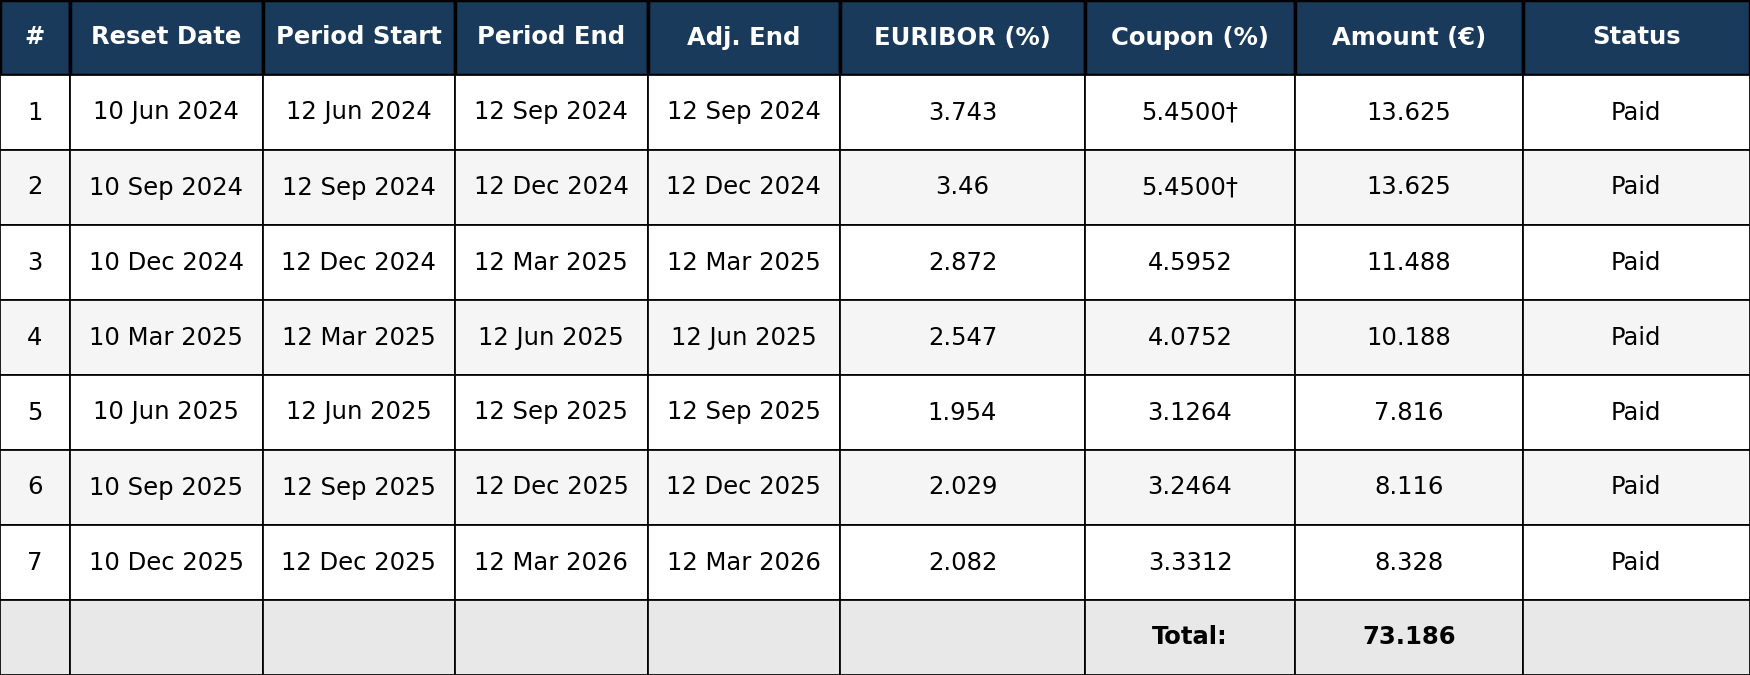
\includegraphics[width=\linewidth,interpolate=true]{coupon_table.png}
  \caption{Coupon schedule per \texteuro{1,000} face value; all dates and amounts generated via QuantLib.}
  \label{fig:coupon_history}
  \vspace{-10pt}
\end{wrapfigure}

Figure~\ref{fig:coupon_history} shows all coupons paid to-date using Bank of Finland
(Suomen Pankki) 3M EURIBOR fixings.\footnote{%
  \url{https://www.suomenpankki.fi/en/Statistics/interest-rates/charts/korot_kuviot/euriborkorot_pv_chrt_en/}}
We use $\alpha = 0.25$ (30/360)
\parencites[App.~B]{BrigoMercurio2006}[Ch.~2]{Fabozzi2012}.
\noindent
Coupons 1,2 were cap-binding ($r =$ 3.743\% and 3.460\%, both above 3.406\%) costing investors approximately \texteuro1.56/\texteuro1{,}000 in upside
(\texteuro1.35 + \texteuro0.22).
ECB rate cuts over 2024--2025 resulted in the reference rate falling $\approx$179~bps, to a trough of 1.954\% (June~2025).
By September--December~2025 the rate recovered to 2.029--2.082\%,
with coupons of 3.246--3.331\% still $\approx$135~bps below the 3.406\% cap break-even.

\subsubsection{Best- and Worst-Case Scenario Analysis}
\label{sssec:scenarios}

We evaluated scenarios by modifying the 3M reference rate but keeping the discount curve fixed:

\begin{itemize}\setlength{\itemsep}{1pt}
  \item \textbf{Best case}-- $r$ stays above the cap break-even (3.406\%) at every future reset, so every coupon pays the maximum 5.45\% p.a.  
  \item \textbf{Base case}-- future reference rates are taken from the forward curve built in our bootstrapping step. We then calculate the coupon using the collar formula (floor at 0\%, cap at 5.45\%, multiplied by 1.60).
  \item \textbf{Worst case}-- $r$ equals 0\% or below at every future reset and every coupon yields 0\%.
    The bondholder will receive only the par amount at maturity.
\end{itemize}
\begin{wraptable}{r}{0.50\textwidth}
  \vspace{-12pt}
  \centering\scriptsize
  \setlength{\tabcolsep}{3pt}
  \begin{tabular}{@{}lrrrr@{}}
    \toprule
    \textbf{Scenario} & \textbf{Cpn PV} & \textbf{Rdm PV}
      & \textbf{Total PV} & \textbf{\% Par} \\
    \midrule
    Best  (cap)    & 420.11 & 802.26 & 1\,222.37 & 122.2\% \\
    Base  (fwd)    & 316.84 & 802.26 & 1\,119.10 & 111.9\% \\
    Worst (floor)  &  16.37 & 802.26 &   818.63  &  81.9\% \\
    \bottomrule
  \end{tabular}
  \vspace{1pt}
  \caption{PV decomposition (per \texteuro1,000 face).}
  \label{tab:q4_scenarios}
  \vspace{-10pt}
\end{wraptable}

\noindent
Table~\ref{tab:q4_scenarios} shows fair values spanning \texteuro819--1,222 ($\approx$40\% of par). The base case yields \texteuro1,119 (112\% of par). Figure~\ref{fig:q4_scenarios} illustrates the cash-flow profiles.

\begin{figure}[htbp]
  \centering
  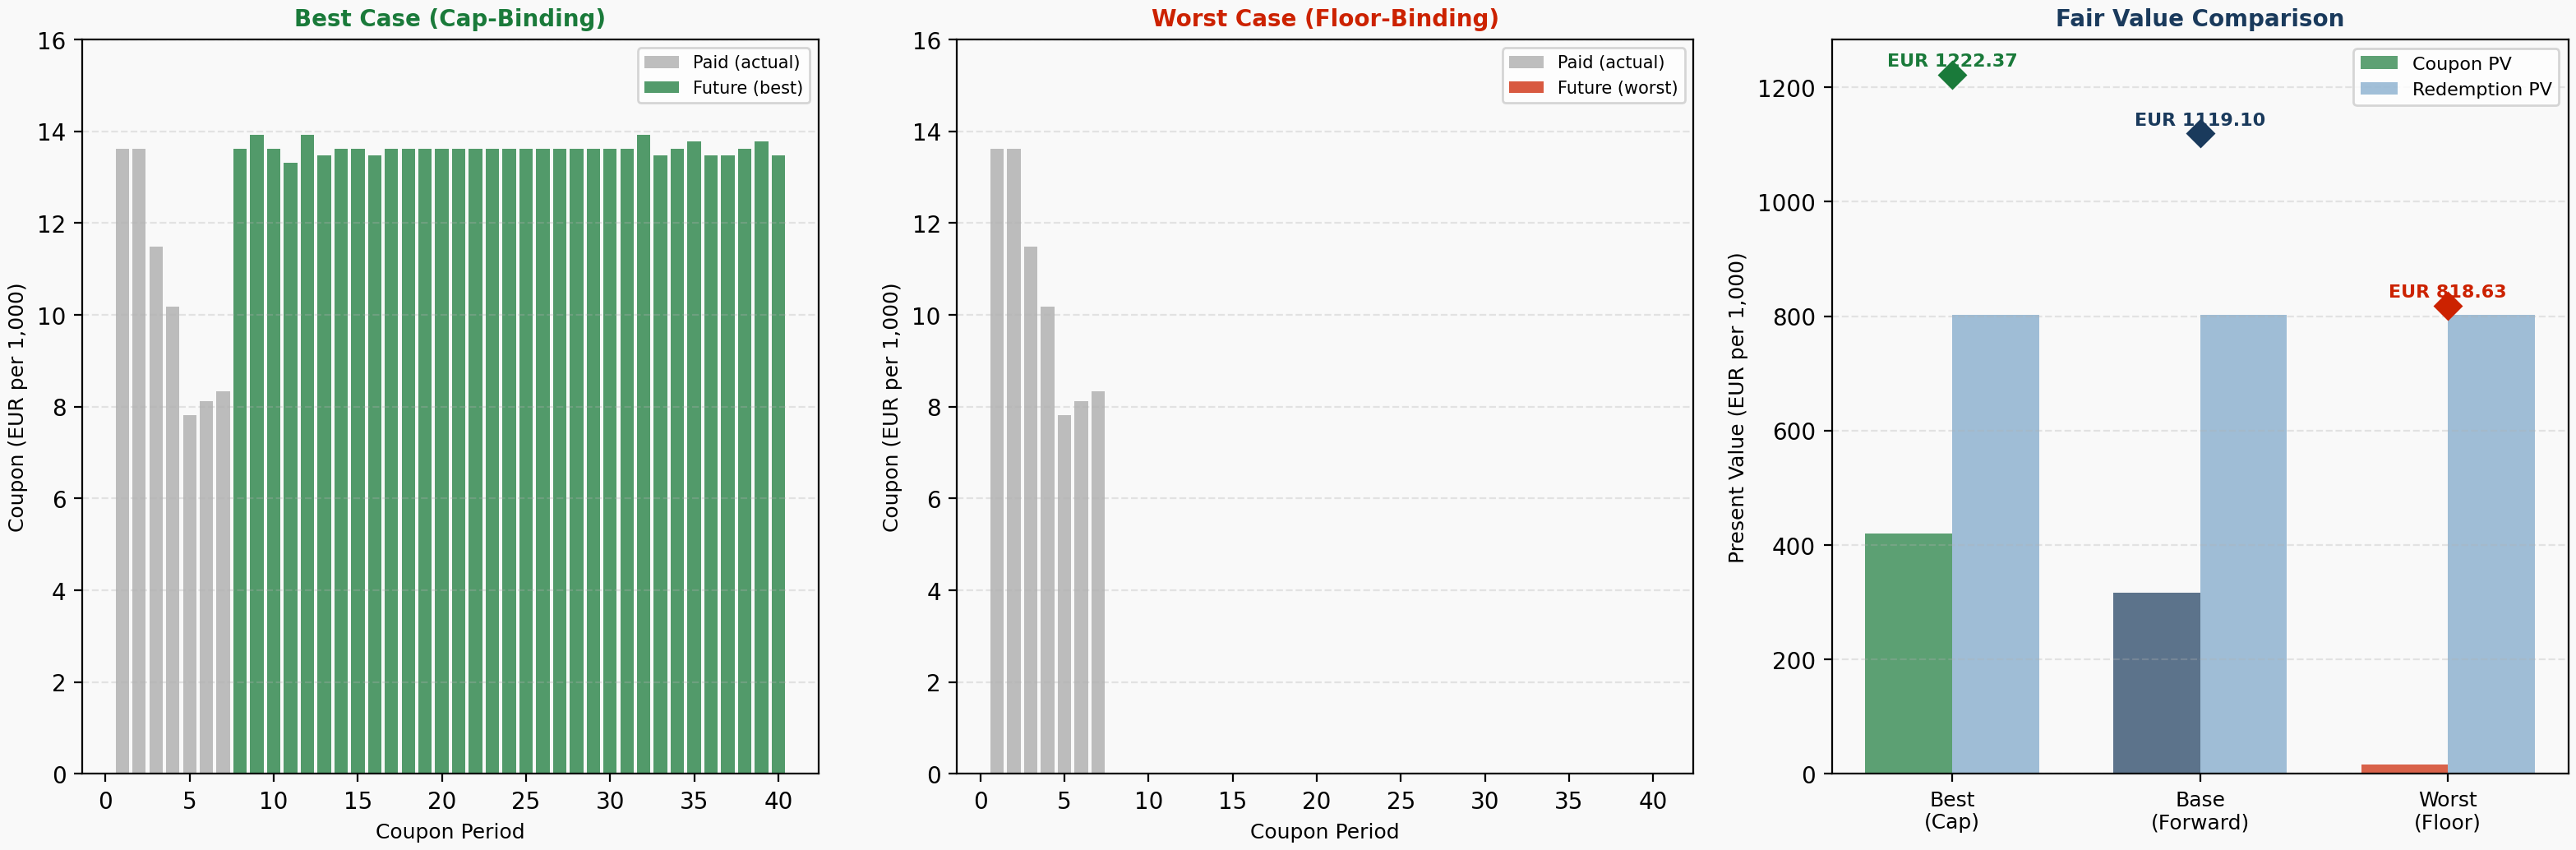
\includegraphics[width=\textwidth]{q4_scenarios.png}
  \caption{Scenario analysis: best/worst coupon cash flows and fair-value comparison.}
  \label{fig:q4_scenarios}
\end{figure}

\subsection{Market Data and Decision-Making}

\subsubsection{Choice of Reference Rate and Data Sources}

The term structure is based on EUR instruments observed on
5~November~2025 (source: LSEG~Refinitiv, dataset \texttt{MarketData202526.xlsx}):

\begin{itemize}[leftmargin=*]\setlength{\itemsep}{1pt}
  \item \textbf{EURIBOR cash deposits} (overnight (O/N)--6M): unsecured interbank rates that yield model-free discount factors at the short end.
  \item \textbf{EUR IRS (AB6E, 1Y--10Y)}: mid par fixed rates vs.\ 6M~EURIBOR (annual fixed 30/360, semi-annual float ACT/360). Bid-offer spreads of 0.1--0.3~bps make these the most liquid long-end EUR rate instruments \parencite[Ch.~2]{Tuckman2011}.
\end{itemize}

\subsubsection{Justification of Market Data Selection}

We use short-term deposits (O/N--6M, settled T+2, ACT/360) because we can calculate a discount factor directly\parencite[p.~92]{Choudhry2010}. We chose to drop the 12M deposit and instead use 1Y~IRS because the swap has tighter bid--offer spreads and we can compute discount factor and  forward rate in one go.

\subsection{Methodologies}

\subsubsection{Bootstrapping Procedure}
\label{sssec:bootstrapping}

We use bootstrapping to build zero-coupon discount-factor curve 
\parencite[Ch.~3]{Choudhry2010}.

\paragraph{Short end: deposits.}
For a deposit with quoted ACT/360 rate $r_d$ and maturity $T$:
\begin{equation}
  DF(T) = \frac{1}{1 + r_d \cdot \alpha},
  \qquad \alpha = \frac{\text{actual days}}{360}
  \label{eq:deposit_df}
\end{equation}
We use four deposits (1W, 1M, 3M, 6M) for maturities of 0.02--0.50 years.

\paragraph{Long end: IRS.}
At inception, fixed leg equals floating leg because a par swap has zero NPV:
\begin{equation}
  c \sum_{i=1}^{n} \alpha^{\text{fix}}_i \, DF(t_i) = DF(t_0) - DF(T_n)
  \label{eq:par_swap}
\end{equation}
where $t_0$ is the settlement date and $\alpha^{\text{fix}}_i = 1$ (annual 30/360
for full coupon years).  Rearranging for the unknown terminal discount factor:
\begin{equation}
  DF(T_n) = \frac{DF(t_0) - c\displaystyle\sum_{i=1}^{n-1}\alpha^{\text{fix}}_i\,DF(t_i)}
                 {1 + c\,\alpha^{\text{fix}}_n}
  \label{eq:bootstrap_irs}
\end{equation}
All prior $DF(t_i)$ are known and each new maturity adds
exactly one equation and one unknown, so the system is solved sequentially without iteration \parencite[p.~437]{Hull2022}.
We implement in QuantLib via \texttt{ql.DepositRateHelper} and
\texttt{ql.SwapRateHelper} combined in a
\texttt{ql.PiecewiseLogLinearDiscount} term structure.

\subsubsection{Interpolation Methods}

For a date $t$ between pillars $T_1$ and $T_2$:
\begin{equation}
  \ln DF(t) = \ln DF(T_1)
  + \frac{t-T_1}{T_2-T_1}\bigl[\ln DF(T_2) - \ln DF(T_1)\bigr]
  \label{eq:loglin}
\end{equation}
This is algebraically equivalent to assuming a \emph{piecewise-constant
instantaneous forward rate} $f_{[T_1,T_2]}$ between each pair of adjacent pillars:
\begin{equation}
  f_{[T_1,T_2]} = \frac{\ln DF(T_1) - \ln DF(T_2)}{T_2 - T_1}
  \label{eq:fwd_const}
\end{equation}

We chose Log-linear interpolation for three
reasons \parencite{HaganWest2006}:
\begin{enumerate}\setlength{\itemsep}{1pt}
  \item since $DF$ is monotonically
    decreasing, $f_{[T_1,T_2]} > 0$ is guaranteed at all inter-pillar dates.
  \item a change in one pillar quote affects only the
    two adjacent intervals, not the entire curve.
  \item no root-finding between pillars;
    a single log-linear formula suffices.
\end{enumerate}
The step-like pattern in the 3M forward curve (Figure~\ref{fig:q3_curves},
panel~2) is a result of the piecewise-constant forward
assumption. A Monte~Carlo comparison of term-structure estimation techniques by \textcite{BiuonoGregoryAllen1992} found that exponential-spline and
piecewise-linear methods deliver similar accuracy at typical market data
densities, justifying our selection to use simpler log-linear approach.

\begin{figure}[htbp]
  \centering
  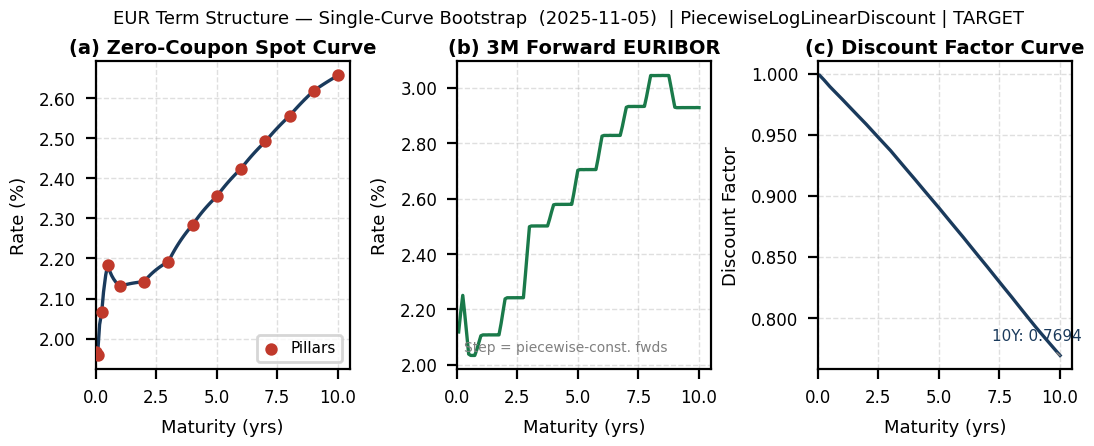
\includegraphics[width=0.95\textwidth]{q3_curves.png}
  \caption{EUR term structure bootstrap (5~Nov~2025): (a)~zero-coupon spot curve, (b)~3M forward EURIBOR, (c)~discount factors.}
  \label{fig:q3_curves}
\end{figure}

\subsubsection{Curve Construction and Validation}

We observe the bootstrapped curve has 15 nodes and spans 0.01-10.25 years. Selected zero rates and discount factors are summarised in Table~\ref{tab:q3_zero_rates} and in  Figure~\ref{fig:q3_curves}.
\noindent
We have validated that every input instrument reprices to within 0.0000~bps (Figure~\ref{fig:q3_validation}), the theoretical minimum for an exact single-curve bootstrap.  The curve is upward-sloping with a mild positive
convexity between 1Y and 10Y while longer maturities reflected a gradual return to neutral
\parencite[Ch.~5]{Tuckman2011}.
\section{Pricing Procedures and Model Justification}

\subsection{Pricing Procedures}
% Outline the procedures adopted for pricing.

\subsubsection{Decomposition into Replicating Instruments}

Using Equation~\eqref{eq:decomposition}, the option-like part of the coupon is
valued as a strip of quarterly floorlets and caplets on 3M~EURIBOR with
effective notional $N^* = 1.60\times N$:
\begin{equation}
  c(r) = 1.60r + \max(0-1.60r,0) - \max(1.60r-5.45\%,0)
  \label{eq:q5_coupon_decomp}
\end{equation}
Hence, for valuation at $t_0$,
\begin{equation}
  PV_{\text{opt}}(t_0) = \sum_i PV(\text{floorlet}_i) - \sum_i PV(\text{caplet}_i),
  \label{eq:q5_opt_pv}
\end{equation}
with floor strike $K_F=0\%$ and cap strike on EURIBOR
$K_C=5.45\%/1.60=3.40625\%$.

\noindent
\begin{minipage}[t]{0.42\textwidth}
  \vspace{0pt}
  \setlength{\tabcolsep}{4pt}
  \centering\scriptsize
  \begin{tabular}{@{}lrrr@{}}
    \toprule
    \textbf{Maturity} & \textbf{DF} & \textbf{Zero (ann.\%)} & \textbf{Fwd 3M (\%)} \\
    \midrule
    1Y  & 0.9793 & 2.131 & 2.105 \\
    2Y  & 0.9586 & 2.142 & 2.238 \\
    3Y  & 0.9370 & 2.192 & 2.498 \\
    5Y  & 0.8902 & 2.355 & 2.702 \\
    7Y  & 0.8418 & 2.492 & 2.929 \\
    10Y & 0.7694 & 2.657 & 2.928 \\
    \bottomrule
  \end{tabular}
  \vspace{2pt}
  \captionof{table}{Bootstrapped zero rates and discount factors
    at key maturities (5~Nov~2025).}
  \label{tab:q3_zero_rates}
\end{minipage}%
\hfill
\begin{minipage}[t]{0.55\textwidth}
  \vspace{0pt}
  \centering
  \includegraphics[width=\linewidth]{q3_validation.png}
  \captionof{figure}{Bootstrap validation: input vs.\ curve-implied rates.
    Maximum absolute error: 0.0000~bps across all 14 instruments.}
  \label{fig:q3_validation}
\end{minipage}

% ────────────────────────────────────────────────────────────────────────────


\subsubsection{Discounting and Forward Rate Estimation}

Discount factors and forwards are taken from the Q3 term structure
(Section~\ref{sssec:bootstrapping}), built from EUR deposits and AB6E swaps on
5~Nov~2025. For each coupon period $[T_{i-1},T_i]$ we use simple forward $F_i$ from the curve and use
$\alpha_i^{30/360}$. 

\subsubsection{Cap and Floor Pricing via Black-76 / Bachelier Model}
\label{sssec:capfloor}
\label{ssec:q5_option_val}

We implement Bachelier (normal) model consistent with the
market sheet \texttt{Bachelier} in \newline
\texttt{MarketData202526.xlsx}. 
For each optionlet with expiry \(\tau_i\), forward \(F_i\), strike \(K\), and
normal volatility \(\sigma_i^N\), the unit payoff price is:
\begin{equation}
  V_i^{\text{Bach}} = \text{BachCall/Put}(F_i,K,\sigma_i^N\sqrt{\tau_i}),
  \label{eq:q5_bachelier_unit}
\end{equation}
and the cashflow PV is:
\begin{equation}
  PV_i = N^*\,\alpha_i^{30/360}\,DF(t_0,T_i)\,V_i^{\text{Bach}}.
  \label{eq:q5_bachelier_cf}
\end{equation}

we then calibrate in two steps:
\begin{enumerate}\setlength{\itemsep}{1pt}
  \item Read ATM 6M EUR cap quotes (maturities 1Y to 10Y) from the market
  workbook.
  \item We extract the implied normal volatility for each individual caplet, one maturity at a time, by matching the cap's weighted variance
  \begin{equation}
    \sigma_{\text{cap}}(T_n)^2 A_n = \sum_{j=1}^{n} w_j\,\sigma_j^2,
    \qquad
    w_j = \alpha_j^{\text{ACT/360}} DF(t_0,T_j),
    \label{eq:q5_strip}
  \end{equation} 
\end{enumerate}


\subsection{Model Justification}
% Provide a rationale for the chosen pricing models.

\subsubsection{Choice of Interest Rate Model}

\begin{wraptable}[8]{r}{0.48\textwidth}
  \vspace{-12pt}
  \centering\small
  \begin{tabular}{@{}lr@{}}
    \toprule
    \textbf{Component} & \textbf{PV (\texteuro/1\,000)} \\
    \midrule
    Long floorlet strip PV & 3.0586 \\
    Short caplet strip PV  & 31.5886 \\
    Net option PV (floor $-$ cap) & $-$28.5300 \\
    \bottomrule
  \end{tabular}
  \vspace{2pt}
  \caption{Option component PV (5~Nov~2025).}
  \label{tab:q5_option_pv}
  \vspace{-10pt}
\end{wraptable}

Since the coupon
(Equation~\eqref{eq:coupon_formula}) depends only on 3M~EURIBOR caplet
fixings, we price each caplet directly under the Bachelier (normal)(Section~\ref{sssec:capfloor}). We used discount factors from Section~\ref{sssec:bootstrapping}.  We preferred this cap--floor approach over leveraged-collar structure because it is
arbitrage-free and consistent with quoted market
prices \parencite[Ch.~29]{Hull2022}.


\section{Implementation of Pricing Procedure}

\subsection{Implementation Overview}

\subsubsection{Yield Curve Construction in QuantLib}

We implement the bootstrapping system as in equations~\eqref{eq:deposit_df}--\eqref{eq:bootstrap_irs}
using QuantLib via \texttt{Piecewise\-LogLinear\-Discount}.
The curve construction is implemented in \texttt{Q3/q3\_main.py};
Table~\ref{tab:q3_zero_rates} and Figure~\ref{fig:q3_curves} present
the resulting zero rates, 3M forward rates, and discount factors.

\subsubsection{Coupon Schedule and Cash Flow Generation}

Coupon dates are generated with QuantLib under TARGET calendar,
Modified-Following convention, quarterly frequency, and 30/360 BondBasis day
count. Reset dates are set to two TARGET business days before each period start.
Only periods with reset date strictly after valuation date contribute option
value in Q5.


\subsubsection{Valuation of Embedded Options}

Embedded options are valued in \texttt{Q5/q5\_main.py}. The implementation:
\begin{enumerate}\setlength{\itemsep}{1pt}
  \item loads ATM cap quotes from the Bachelier sheet,
  \item strips caplet normal vols by sequential variance matching,
  \item prices each caplet/floorlet with QuantLib's Bachelier formula,
\end{enumerate}
\subsubsection{CVA Computation}
\label{sssec:cva_impl}

We compute CVA in \texttt{Q6/q6\_main.py}.
The implementation:
\begin{enumerate}\setlength{\itemsep}{1pt}
  \item builds the 40-period coupon schedule and projects base-case cash
    flows using historical fixings (periods~1--7) and Q3 forward rates
    (periods~8--40), applying the leveraged-collar formula,
  \item adds the \EUR{1,000} par redemption at maturity,
  \item constructs a flat-hazard survival curve from the 5-year CDS spread
    ($s = 75$~bps, $R=40\%$, $\lambda=125$~bps/yr),
  \item at each future coupon date $T_i$, computes expected exposure
    (PV of remaining flows) and marginal default probability
    $Q(T_{i-1})-Q(T_i)$
\end{enumerate}

\subsubsection{Fair Value Assembly}
\label{sssec:q8_impl}

We construct the full decomposition table texttt{Q8/q8\_main.py}.
The script:
\begin{enumerate}\setlength{\itemsep}{1pt}
  \item computes the leveraged FRN leg PV (uncollared: $1.60 \times F_i
    \times \alpha_i \times DF_i$ for each future period),
  \item reads Q5 option component PVs from
    \texttt{q5\_option\_components.csv},
  \item recomputes the CVA using the same flat-hazard model as Q6,
  \item calculates accrued interest for the current coupon period
    (30/360 BondBasis from period start to evaluation date)
\end{enumerate}


\section{Results and Discussion}

\subsection{Results}
% Present the results obtained.

\subsubsection{Fair Value Decomposition}

We priced the embedded options using the calibrated Bachelier model across
the 34 future coupon periods (7--40, Dec~2025 to Jun~2034).
Table~\ref{tab:q5_option_pv} gives the per-period breakdown.

\needspace{10\baselineskip}
\begin{wraptable}{r}{0.52\textwidth}
  \vspace{-10pt}
  \centering\small
  \begin{tabular}{@{}lr@{}}
    \toprule
    \textbf{Component} & \textbf{PV (\texteuro/1\,000)} \\
    \midrule
    Long floor ($K_f = 0\%$)  & 3.0586 \\
    Short cap ($K_c = 3.41\%$) & 31.5886 \\
    \midrule
    \textbf{Net option value} & \textbf{$-$28.5300} \\
    \bottomrule
  \end{tabular}
  \vspace{2pt}
  \caption{Aggregate embedded-option PV.}
  \label{tab:q5_agg_option}
  \vspace{-10pt}
\end{wraptable}

Table~\ref{tab:q5_agg_option} shows that the net option value is
negative: the sold cap is worth far more than the purchased floor.
Because the cap strike $K_c \approx 3.41\%$ sits just above current
3M~EURIBOR forwards ($\approx 2$--$3\%$), the short caplets carry
significant value.  The zero-strike floor is deep out-of-the-money, so
its \EUR{3.06} PV is nearly all time value.

We also observe that the option cost rises with maturity.  Early
periods (7--10) contribute little, while the final periods (39--40)
each add roughly \EUR{2.1} on the cap side.  This pattern reflects
(i)~rising stripped caplet vols (27.5~bps at 1Y to 73.1~bps at 10Y)
and (ii)~increasing forward rates along the curve.

\subsubsection{Credit Valuation Adjustment}
\label{sssec:cva_results}

\begin{wraptable}{r}{0.50\textwidth}
  \vspace{-10pt}
  \centering\small
  \begin{tabular}{@{}lr@{}}
    \toprule
    \textbf{Metric} & \textbf{Value (\texteuro/1\,000)} \\
    \midrule
    Risk-free bond PV         & 1\,119.32 \\
    CVA                       & 59.43 \\
    \textbf{Risky bond PV}    & \textbf{1\,059.89} \\
    \midrule
    CVA as \% of notional     & 5.94\% \\
    CVA as \% of risk-free PV & 5.31\% \\
    \bottomrule
  \end{tabular}
  \vspace{2pt}
  \caption{CVA summary (CDS 75~bps, $R\!=\!40\%$).}
  \label{tab:q6_cva}
  \vspace{-10pt}
\end{wraptable}

Table~\ref{tab:q6_cva} shows our CVA results.  Using the flat-hazard
model, we find a CVA of \EUR{59.43} per \EUR{1\,000} notional, which
brings the risk-free value of \EUR{1,119.32} down to a credit-risky
value of \EUR{1,059.89}.  The expected exposure falls steadily from
\texteuro1,119 at the first future coupon to \texteuro812 at the final
period, as remaining cash flows shrink with each payment.  Because the
quarterly default probability stays roughly constant at $\approx$0.31\%,
earlier periods—where exposure is highest—contribute slightly more to
the total CVA.

\subsubsection{Comprehensive Fair Value Table}
\label{sssec:q8_results}

\begin{wraptable}{r}{0.55\textwidth}
  \vspace{-10pt}
  \centering\small
  \begin{tabular}{@{}lrr@{}}
    \toprule
    \textbf{Component} &
    \textbf{PV (EUR)} &
    \textbf{\% par} \\
    \midrule
    A.~Leveraged FRN leg
      & 317.06 & 31.71 \\
    B.~Long floor strip ($K_F\!=\!0\%$)
      &   3.06 &  0.31 \\
    C.~Short cap strip ($K_C\!=\!3.406\%$)
      & $-$31.59 & $-$3.16 \\
    \quad Net option (B$+$C)
      & $-$28.53 & $-$2.85 \\
    D.~Par redemption
      & 802.26 & 80.23 \\
    \midrule
    \textbf{Risk-free dirty} (A--D)
      & \textbf{1\,119.32} & \textbf{111.93} \\
    E.~CVA
      & $-$59.43 & $-$5.94 \\
    \midrule
    \textbf{Risky dirty} (A--E)
      & \textbf{1\,059.89} & \textbf{105.99} \\
    F.~Accrued interest
      & $-$4.78 & $-$0.48 \\
    \midrule
    \textbf{Risky clean price}
      & \textbf{1\,055.11} & \textbf{105.51} \\
    \bottomrule
  \end{tabular}
  \vspace{2pt}
  \caption{Fair value decomposition (\texteuro/1\,000, 5~Nov~2025).}
  \label{tab:q8_fair_value}
  \vspace{-10pt}
\end{wraptable}

Table~\ref{tab:q8_fair_value} brings together all our pricing
components into one decomposition.  We can trace the bond's value from
its building blocks i.e. leveraged FRN leg, option strips, and par redemption through the risk-free dirty price, the CVA deduction, and finally the risky clean price.  The par redemption PV (80.2\% of par)
is the largest piece, followed by the FRN leg (31.7\%).  The net option
cost ($-$2.85\%) and the CVA ($-$5.94\%) together reduce value by about 8.8\%.

Our model-implied risky clean price of \texteuro1,055.11 (105.51\% of par)
is what we estimate an investor should pay on 5~November~2025, before
any transaction costs or liquidity premia.

\subsubsection{Expected Cash Flows}
\label{sssec:q9_cashflows}

Figure~\ref{fig:q9_cashflows} shows the bond's cash flows in three
panels.  Panel~(a) displays the quarterly coupon payments, separating
the five already-paid coupons from the 35~projected future ones and
the par redemption.  Panel~(b) shows the present value of each future
cash flow alongside a cumulative PV line—we can see the total PV of
\texteuro1,119.32 is largely driven by the par redemption
(\texteuro802.26, or 71.7\%).  Panel~(c) overlays historical
3M~EURIBOR fixings and forward rates, with lines at the floor (0\%)
and cap break-even (3.406\%) to show where the coupon gets capped.

\begin{figure}[htbp]
  \centering
  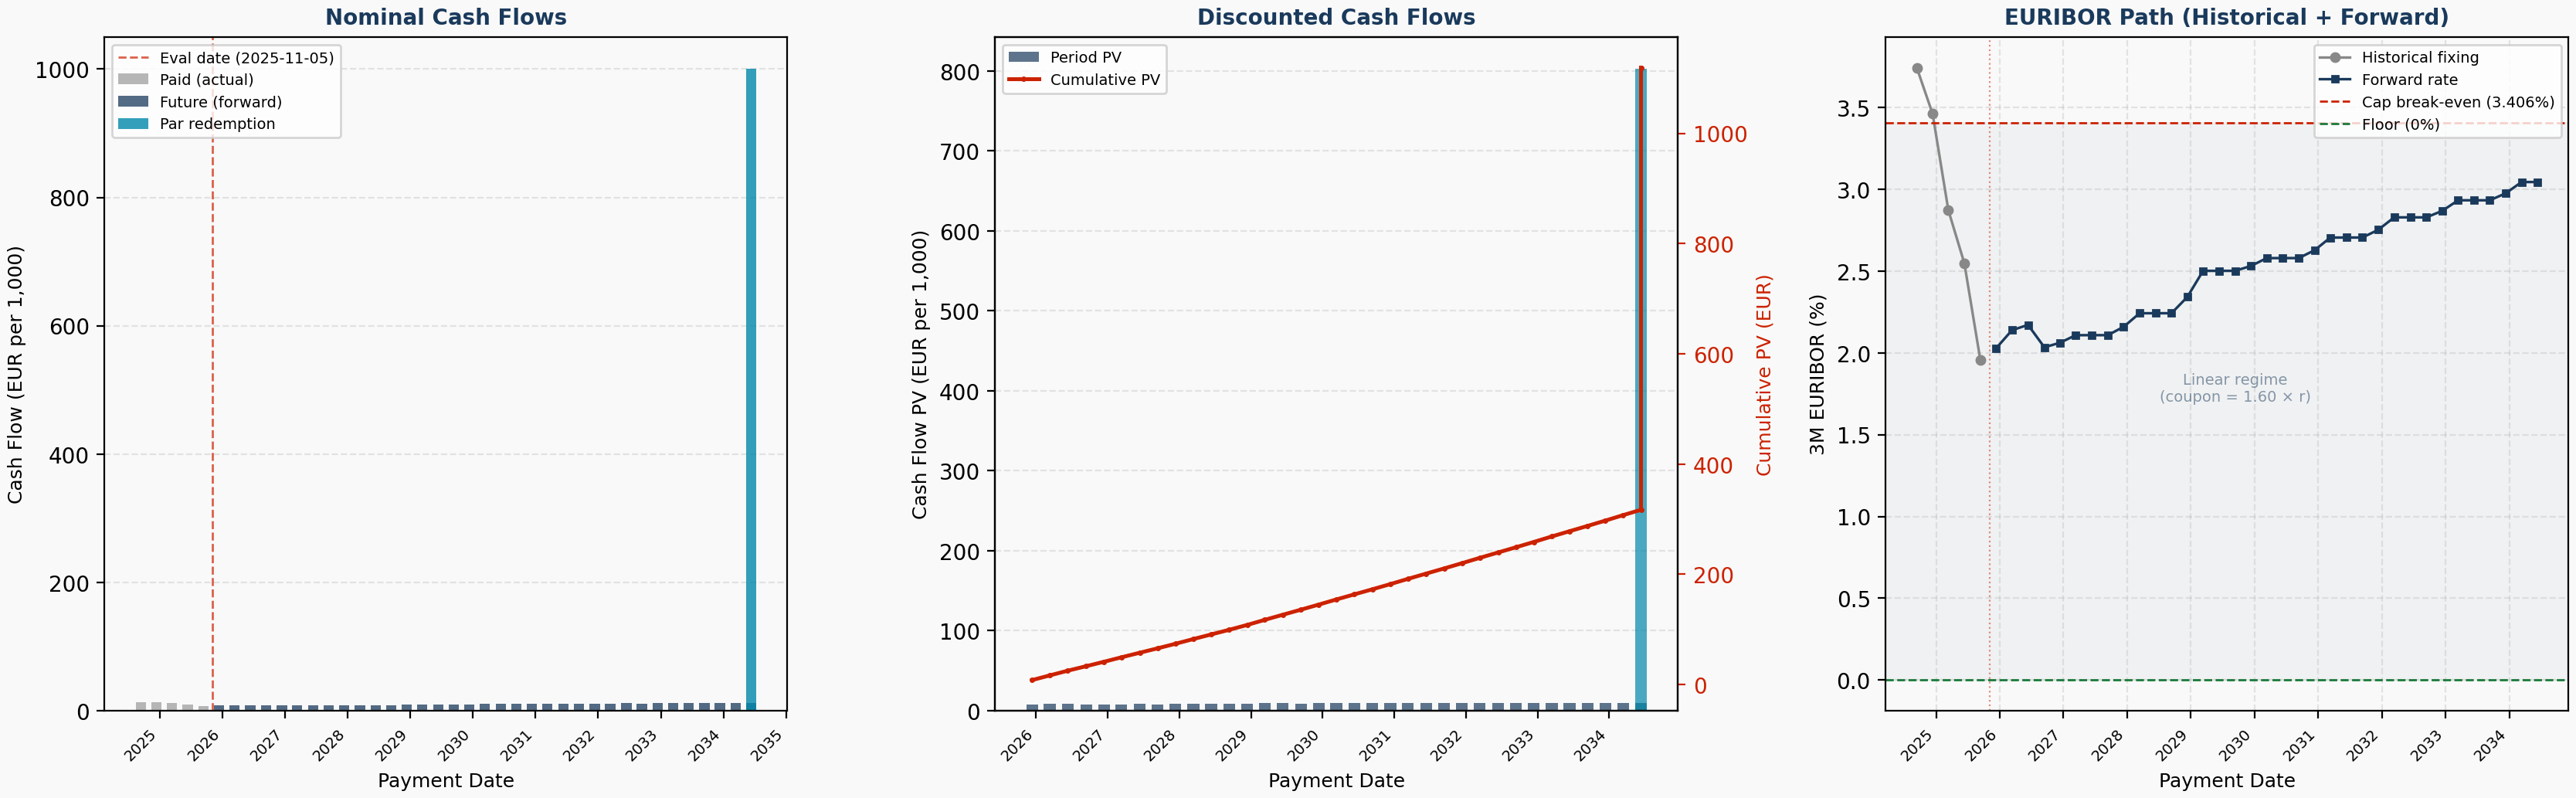
\includegraphics[width=\textwidth]{q9_expected_cashflows.png}
  \caption{Bond expected cash flows (per \texteuro1,000 notional).
    Left: nominal coupons. Centre: period PVs and cumulative PV.
    Right: 3M EURIBOR vs.\ floor/cap thresholds.}
  \label{fig:q9_cashflows}
\end{figure}

The average expected future coupon is 4.044\% (range 3.246--4.870\%),
meaning most coupons fall in the linear part of the structured payoff.
Total nominal future coupons sum to \texteuro353.82, discounting to
\texteuro317.06—matching the FRN-leg value in
Table~\ref{tab:q8_fair_value}.

\subsubsection{Principal Component Analysis of EUR IRS Rates}
\label{sssec:q11_pca}

\begin{wraptable}{r}{0.50\textwidth}
  \centering\small
  \vspace{-10pt}
  \begin{tabular}{@{}lrrrl@{}}
    \toprule
    \textbf{PC} & \textbf{Eigenvalue} & \textbf{Var.~Expl.}
      & \textbf{Cumul.} & \textbf{Interpretation} \\
    \midrule
    PC1 & 113.82 & 91.5\% & 91.5\% & Level \\
    PC2 &   6.97 &  5.6\% & 97.1\% & Slope \\
    PC3 &   1.28 &  1.0\% & 98.1\% & Curvature \\
    \bottomrule
  \end{tabular}
  \vspace{2pt}
  \caption{PCA eigenvalues and variance explained (EUR IRS 1Y--10Y,
    Dec~2015--Dec~2025, 2,609 obs.).}
  \label{tab:q11_pca}
  \vspace{-10pt}
\end{wraptable}

To understand what drives EUR swap-curve movements, we run PCA on
daily first-differences of EUR IRS par rates (1Y--10Y) over
December~2015 to December~2025 (2,609 observations).
We stack the daily changes $\Delta r_{t,k}$ (in~bps) into a matrix
$\mathbf{X}$, compute its covariance
$\boldsymbol{\Sigma}=\mathbf{X}^{\!\top}\mathbf{X}/(T{-}1)$, and
solve the eigenvalue problem
\parencite[Ch.~4]{Tuckman2011}:
\begin{equation}
  \boldsymbol{\Sigma}\,\mathbf{v}_k = \lambda_k\,\mathbf{v}_k,
  \qquad k = 1,\ldots,K.
  \label{eq:q11_pca}
\end{equation}
Each eigenvector $\mathbf{v}_k$ is a principal component, and
$\lambda_k/\sum_j\lambda_j$ gives its share of total variance.
Table~\ref{tab:q11_pca} shows that three PCs capture 98.1\% of
daily rate variation.

Figure~\ref{fig:q11_pca} presents three panels.
Panel~(a) confirms PC1 alone explains 91.5\% of variance---parallel
shifts dominate, as expected for developed-market curves.
Panel~(b) shows loadings: PC1 is flat across tenors (level), PC2
falls from short to long (slope), and PC3 dips in the belly
(curvature).  Panel~(c) tracks cumulative scores, clearly picking up
the 2022--23 hiking cycle and subsequent ECB easing.

\begin{figure}[htbp]
  \centering
  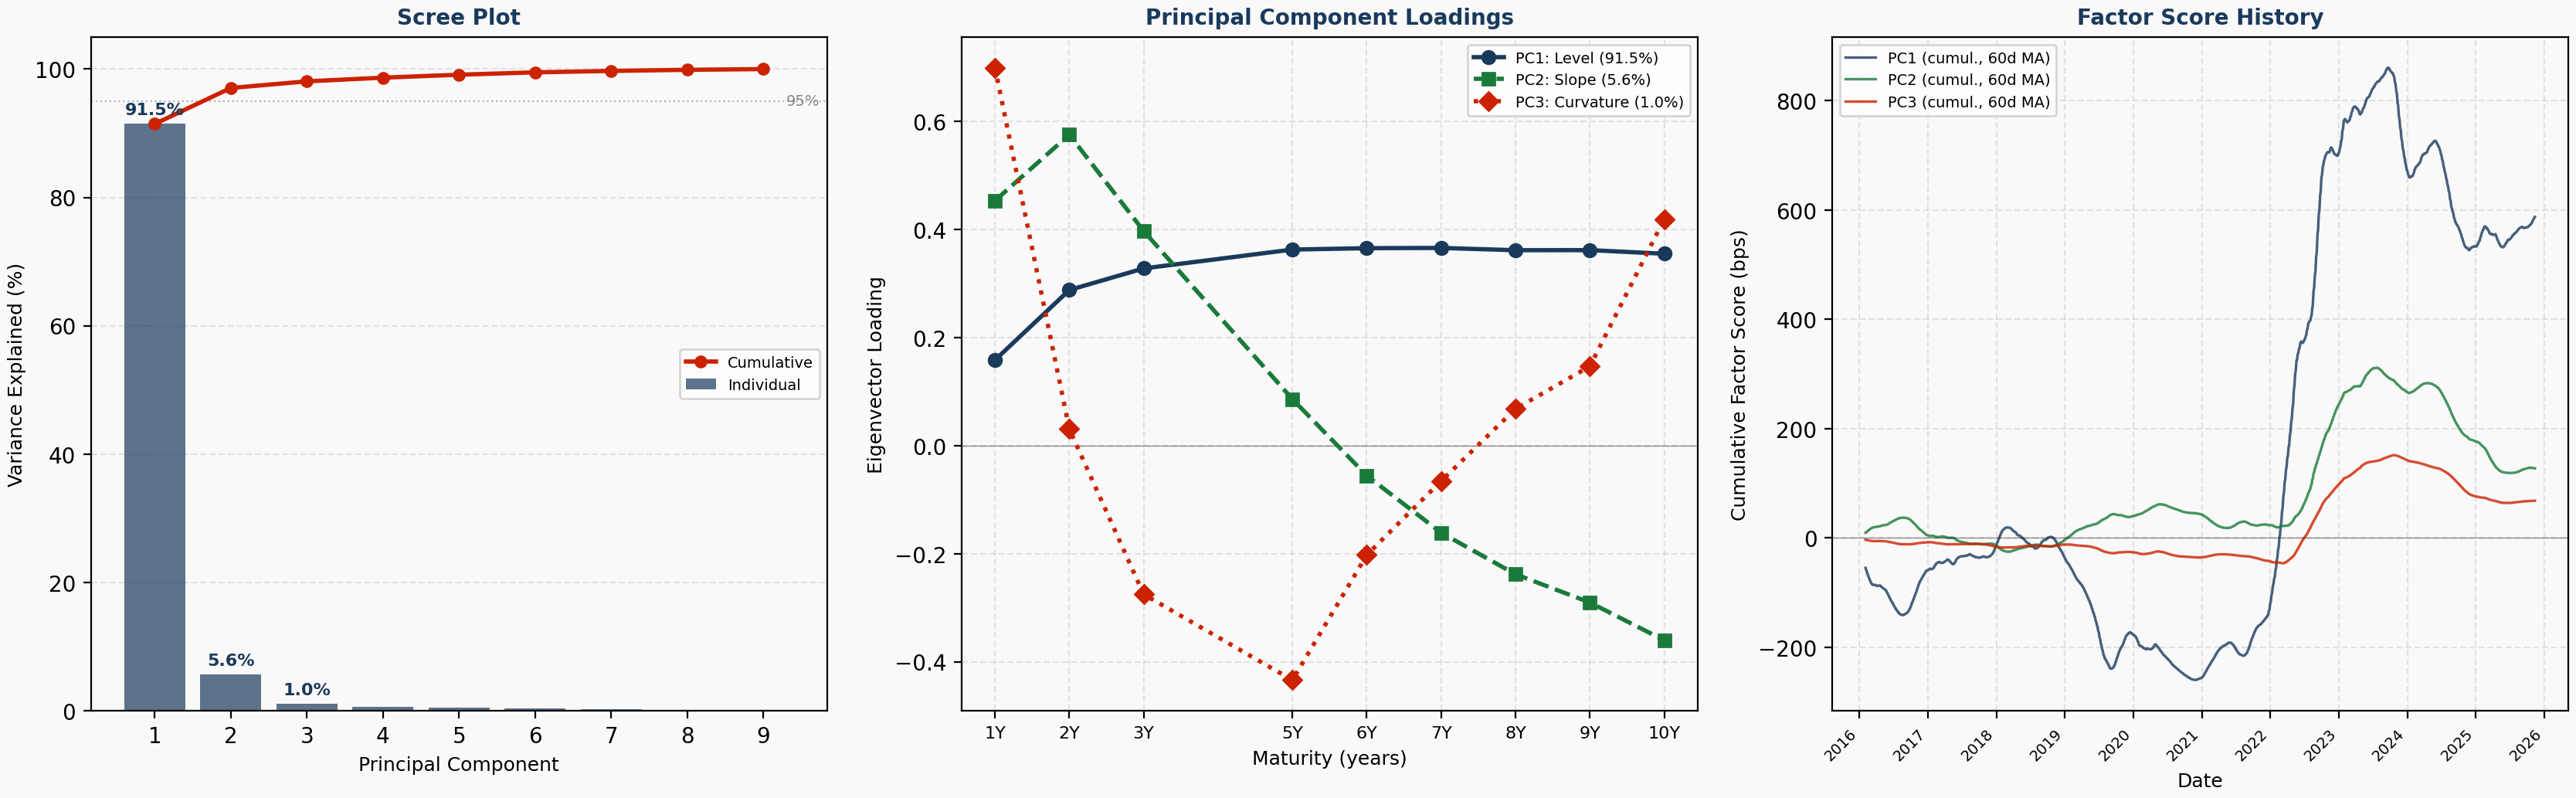
\includegraphics[width=\textwidth]{q11_pca_chart.png}
  \caption{PCA of EUR IRS daily rate changes (1Y--10Y).
    (a)~Scree plot showing variance explained by each PC.
    (b)~Eigenvector loadings for the first three components.
    (c)~Cumulative factor scores (60-day moving average).}
  \label{fig:q11_pca}
\end{figure}

\subsubsection{Sensitivity to Term-Structure Shifts}
\label{sssec:q12_sensitivity}

We now shock the EUR IRS curve along each of the first three PCs and
re-price the bond to measure its level, slope, and curvature exposure.

For each PC$_k$ we apply $\pm 1\sigma$ and $\pm 2\sigma$ monthly shocks:
\begin{equation}
  \Delta r(\tau) \;=\; \delta\,\sqrt{\lambda_k}\,\sqrt{21}\,v_k(\tau),
  \qquad \delta \in \{-2,\,-1,\,+1,\,+2\},
  \label{eq:q12_shock}
\end{equation}
where $\sqrt{21}$ converts the daily standard deviation to a one-month
horizon and $v_k(\tau)$ is the eigenvector loading from
Table~\ref{tab:q11_pca}.  The resulting monthly volatilities are
48.9~bps (PC1), 12.1~bps (PC2), and 5.2~bps (PC3). For each shocked 
curve we re-bootstrap discount factors
, recompute forward EURIBOR
projections, reprice the cap/floor strips
, and update the CVA
.  Accrued interest stays the same since the
current coupon is already fixed.

\paragraph{Results.}

\begin{wraptable}{r}{0.48\textwidth}
  \centering\footnotesize
  \vspace{-12pt}
  \setlength{\tabcolsep}{3pt}
  \begin{tabular}{@{}llrrrr@{}}
    \toprule
    \textbf{PC} & \textbf{Shock} & \textbf{Clean}
      & \textbf{$\Delta$EUR} & \textbf{$\Delta$\%}
      & \textbf{Cl.\%} \\
    \midrule
    \multicolumn{2}{@{}l}{Base} & 1\,055.11 & --- & --- & 105.51 \\
    \midrule
    PC1 & $-2\sigma$ & 1\,040.00 & $-$15.10 & $-$1.51 & 104.00 \\
        & $-1\sigma$ & 1\,048.00 & $-$7.10  & $-$0.71 & 104.80 \\
        & $+1\sigma$ & 1\,061.31 & $+$6.20  & $+$0.62 & 106.13 \\
        & $+2\sigma$ & 1\,057.24 & $+$2.13  & $+$0.21 & 105.72 \\
    \midrule
    PC2 & $-2\sigma$ & 1\,057.86 & $+$2.75 & $+$0.28 & 105.79 \\
        & $-1\sigma$ & 1\,056.48 & $+$1.38 & $+$0.14 & 105.65 \\
        & $+1\sigma$ & 1\,053.73 & $-$1.38 & $-$0.14 & 105.37 \\
        & $+2\sigma$ & 1\,052.35 & $-$2.75 & $-$0.28 & 105.24 \\
    \midrule
    PC3 & $-2\sigma$ & 1\,054.65 & $-$0.46 & $-$0.05 & 105.46 \\
        & $-1\sigma$ & 1\,054.88 & $-$0.23 & $-$0.02 & 105.49 \\
        & $+1\sigma$ & 1\,055.34 & $+$0.23 & $+$0.02 & 105.53 \\
        & $+2\sigma$ & 1\,055.56 & $+$0.46 & $+$0.05 & 105.56 \\
    \bottomrule
  \end{tabular}
  \vspace{2pt}
  \caption{Risky clean price under PCA shocks
    (1-month; base \texteuro1,055; 5~Nov~2025).}
  \label{tab:q12_sensitivity}
  \vspace{-10pt}
\end{wraptable}

Table~\ref{tab:q12_sensitivity} shows the risky clean price under
each scenario.  Figure~\ref{fig:q12_bars} groups the impact by PC,
and Figure~\ref{fig:q12_components} breaks the $\pm 1\sigma$ effects
into their pricing components.
We note three key features.
\textbf{1:} a $+1\sigma$ parallel move (48.9~bps)
raises the price by \texteuro6.20, while $-1\sigma$ lowers it by
\texteuro7.10.  This asymmetry is due to the embedded cap---at
$+2\sigma$ coupons hit the cap region, capping the upside.
\textbf{2:} a $+1\sigma$ steepening (PC2) lowers
the price by \texteuro1.38 as long-end discounting rises faster than
short-end coupon projections.
\textbf{3:} $\pm 1\sigma$ PC3 shifts the price
by only \texteuro0.23 ($\approx$0.02\% of par), since the belly
loadings barely touch the bond's key risk points (3M reset, 8.6Y
redemption).

\begin{figure}[htbp]
  \centering
  \begin{minipage}[t]{0.54\textwidth}
    \centering
    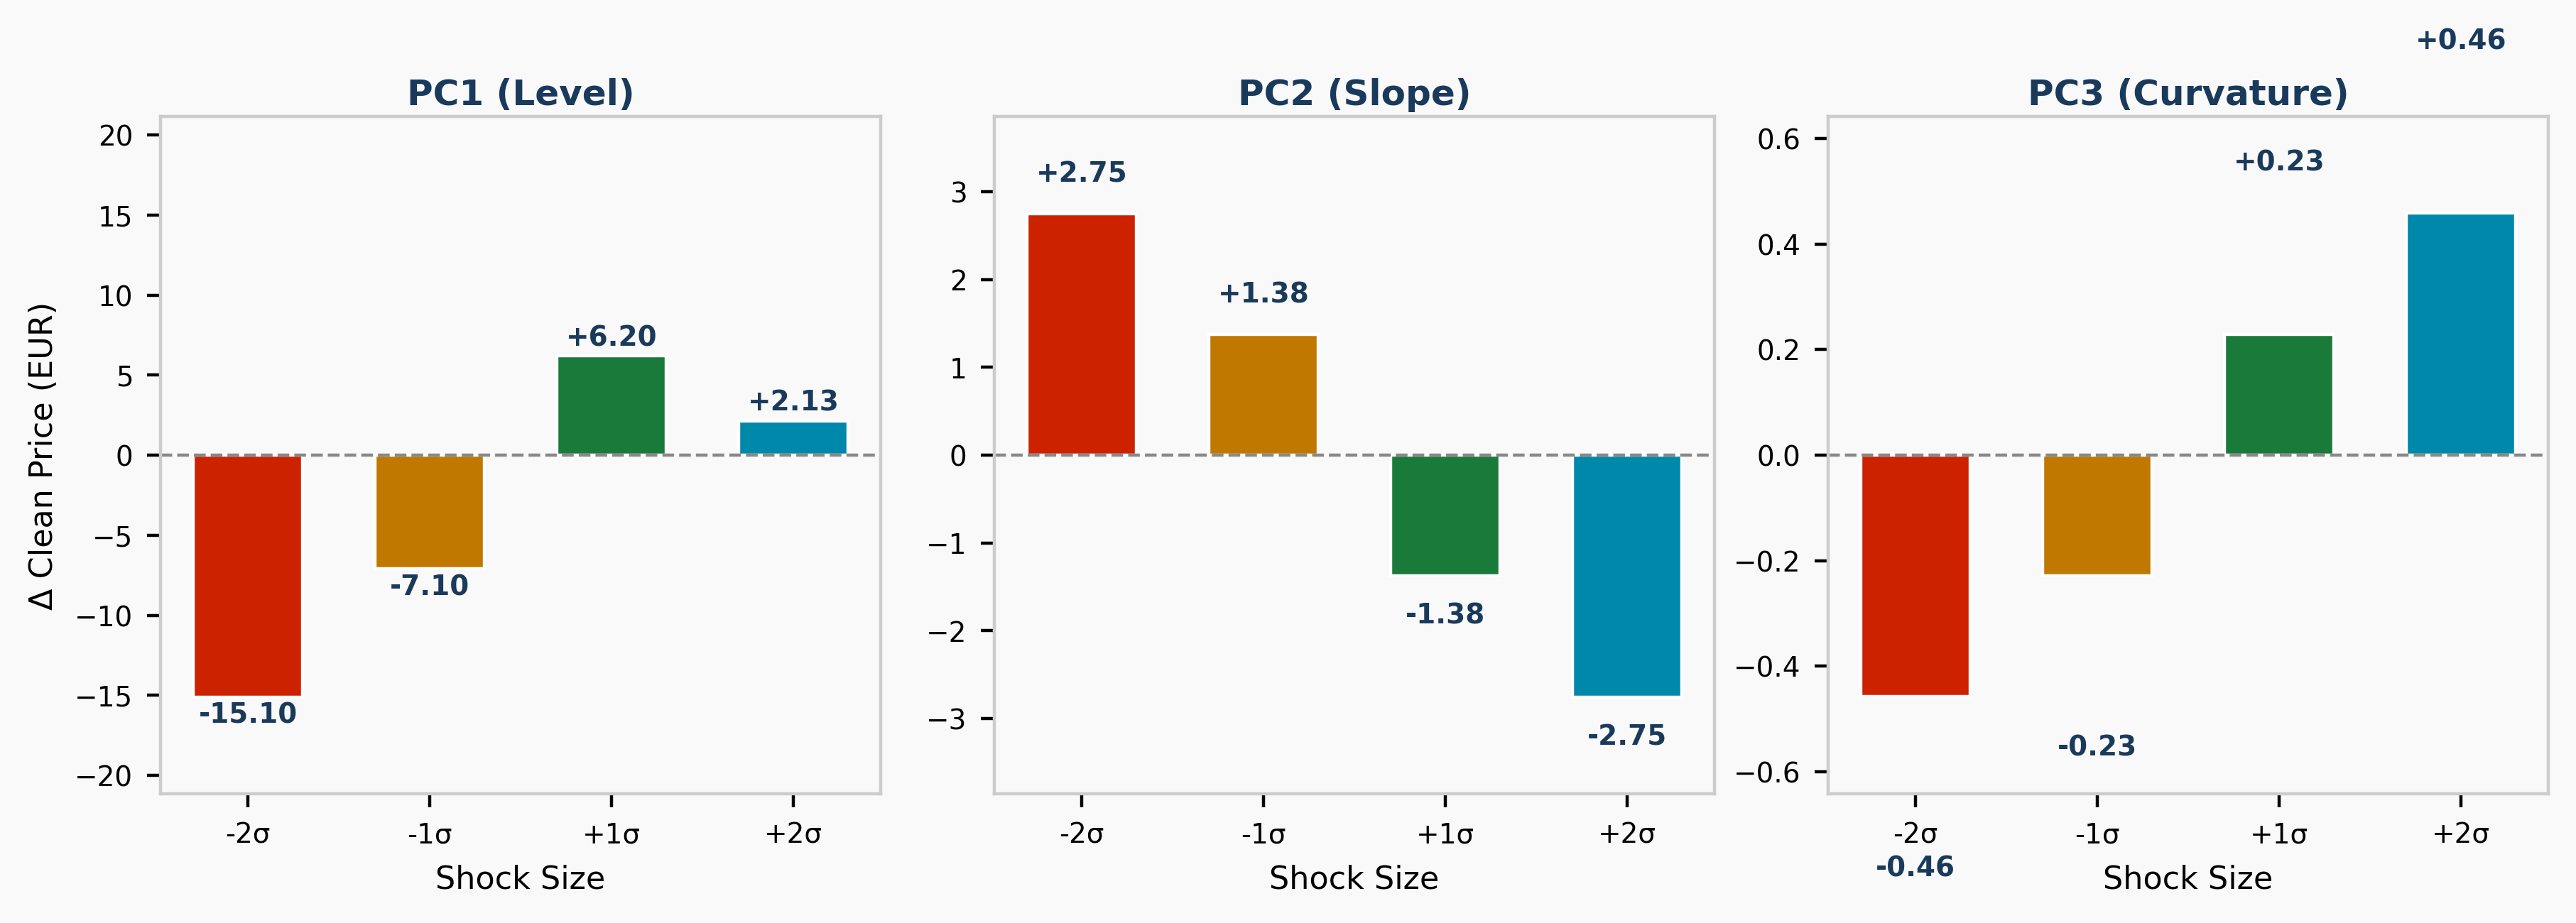
\includegraphics[width=\textwidth]{q12_sensitivity_chart.png}
    \captionof{figure}{Sensitivity of the risky clean price to PCA-based
      shocks ($\pm 1\sigma$, $\pm 2\sigma$; 1-month horizon).}
    \label{fig:q12_bars}
  \end{minipage}\hfill
  \begin{minipage}[t]{0.44\textwidth}
    \centering
    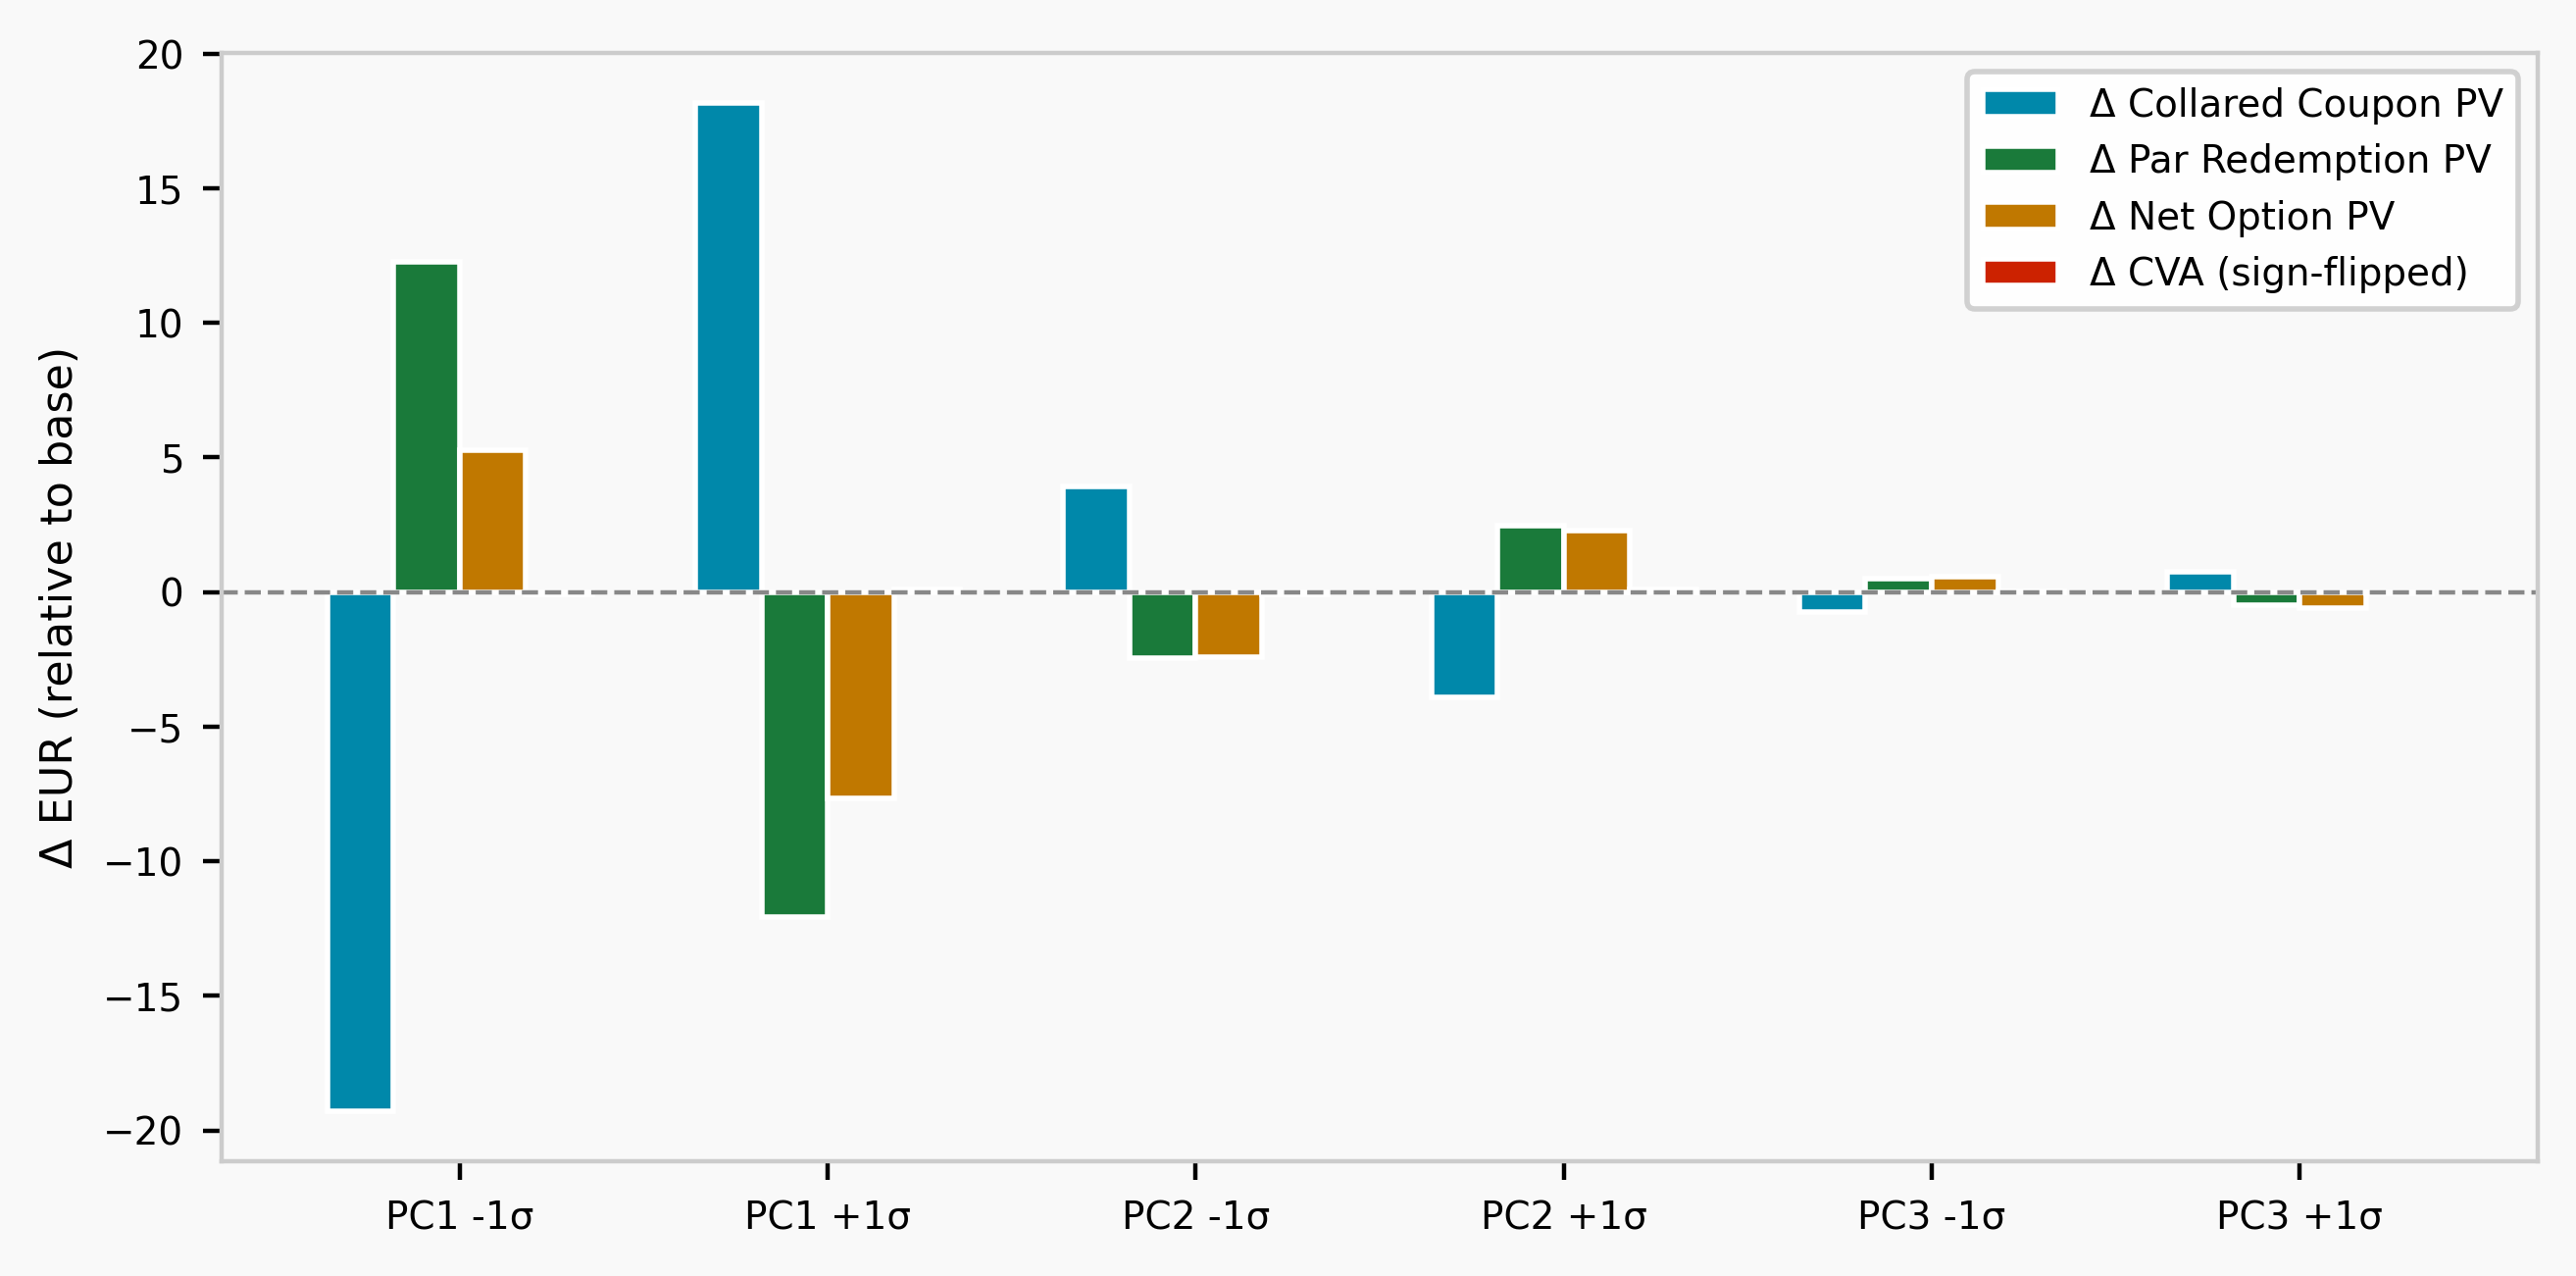
\includegraphics[width=\textwidth]{q12_component_chart.png}
    \captionof{figure}{Component decomposition of price sensitivity
      ($\pm 1\sigma$, 1-month).}
    \label{fig:q12_components}
  \end{minipage}
\end{figure}

\noindent
From Figure~\ref{fig:q12_components} we see that the par-redemption
discount factor drives $\sim$80\% of the PC1 price change.  Coupon PV
moves the other way (higher rates $\Rightarrow$ higher coupons), but
the 1.60$\times$ leverage only partly offsets discounting.  Option
value is stable at $\pm 1\sigma$, yet cap costs jump at
$+2\sigma$---hence the concavity in the PC1 panel of
Figure~\ref{fig:q12_bars}.

\subsubsection{Hedging Strategy with Plain-Vanilla Swaps}
\label{sssec:q13_hedge}

\begin{wraptable}{r}{0.46\textwidth}
  \centering\footnotesize
  \vspace{-12pt}
  \setlength{\tabcolsep}{3pt}
  \begin{tabular}{@{}lrrr@{}}
    \toprule
    \textbf{Factor} & \textbf{Bond} & \textbf{2Y IRS}
      & \textbf{10Y IRS} \\
    & \multicolumn{3}{c}{(EUR / 1~bps move)} \\
    \midrule
    PC1 (Level)     & $+$0.1442 & $-$55.81 & $-$311.25 \\
    PC2 (Slope)     & $-$0.1137 & $-$111.54 & $+$315.85 \\
    PC3 (Curv.)     & $+$0.0441 & $-$5.91  & $-$367.04 \\
    \midrule
    \multicolumn{4}{@{}l}{\textbf{Hedge} (PC1$+$PC2):} \\
    \midrule
    \textbf{Instr.} & \textbf{Dir.}
      & \multicolumn{2}{r}{\textbf{Notional}} \\
    \cmidrule(l){1-4}
    2Y IRS  & Recv & \multicolumn{2}{r}{\texteuro194} \\
    10Y IRS & Recv & \multicolumn{2}{r}{\texteuro429} \\
    \bottomrule
  \end{tabular}
  \vspace{2pt}
  \caption{Factor DV01s and hedge notionals per
    \texteuro1,000 bond notional.}
  \label{tab:q13_dv01}
  \vspace{-10pt}
\end{wraptable}

We hedge the bond's curve exposure with two CCP-cleared EUR AB6E
interest-rate swaps: a \textbf{2Y receiver} and a \textbf{10Y
receiver}.  Two swaps give us two degrees of freedom---enough to
neutralise PC1 (level) and PC2 (slope), which together explain 97.1\%
of curve variance.  IRS are highly liquid, carry minimal counterparty
risk when cleared, and are quoted to the basis point
\parencite[Ch.~7]{Hull2022}.

For each factor $k=1,2$ and instrument $j$ we define the
\emph{factor DV01}:
\begin{equation}
  \mathrm{DV01}_k^{(j)}
    \;=\; \frac{V^{(j)}(\mathbf{r}+\mathbf{v}_k)-V^{(j)}(\mathbf{r}-\mathbf{v}_k)}{2},
  \label{eq:q13_fdv01}
\end{equation}
where $\mathbf{v}_k$ is the unit-bps eigenvector shock and $V^{(j)}$
is the full-repricing function (re-bootstrap $\to$ forwards $\to$
options $\to$ CVA for the bond; standard PV for swaps).

Writing $N_{2}$, $N_{10}$ for the swap notionals, the hedge
condition is:
\begin{equation}
  N_{2}\,\mathrm{DV01}_k^{2\mathrm{Y}}
  + N_{10}\,\mathrm{DV01}_k^{10\mathrm{Y}}
  = -\,\mathrm{DV01}_k^{\mathrm{bond}},
  \qquad k = 1,2.
  \label{eq:q13_hedge}
\end{equation}
Table~\ref{tab:q13_dv01} reports the DV01s and solved notionals.

\paragraph{Verification.}
The hedge zeroes out PC1 and PC2 DV01 completely. The remaining PC3
exposure ($-$0.11~EUR/bps) is tiny---a $\pm 1\sigma$ curvature shock
moves the portfolio by under \texteuro0.60, less than bid--offer costs.

\paragraph{Practical limitations.}
\begin{itemize}[leftmargin=*]\setlength{\itemsep}{1pt}
  \item \textbf{Non-linearity}: the cap creates negative convexity
    for large moves; swaptions would be needed for gamma hedging.
  \item \textbf{Rebalancing}: DV01s drift as rates move, so we must
    rebalance at least monthly.
  \item \textbf{Credit--rate correlation}: we only hedge rate risk;
    credit risk may correlate with rates
    under stress.
  \item \textbf{Basis risk}: the bond resets on 3M~EURIBOR but the
    IRS floats on 6M, leaving a small basis residual.
\end{itemize}

\subsubsection{Hedge Implementation and Performance}
\label{sssec:q14_hedge_impl}

We test the hedge from Section~\ref{sssec:q13_hedge} by repricing the
hedged portfolio (bond $+$ \texteuro194 2Y swap $+$ \texteuro429 10Y swap)
under the twelve PCA scenarios.  The hedged P\&L is simply
$\Delta V_{\text{hedged}} = \Delta V_{\text{bond}}
+ \Delta V_{\text{2Y}} + \Delta V_{\text{10Y}}$.

\begin{wraptable}{r}{0.46\textwidth}
  \centering\scriptsize
  \vspace{-12pt}
  \setlength{\tabcolsep}{2pt}
  \begin{tabular}{@{}llrrrr@{}}
    \toprule
    \textbf{PC} & \textbf{Shock}
      & \textbf{$\Delta$Bond} & \textbf{$\Delta$2Y}
      & \textbf{$\Delta$10Y} & \textbf{$\Delta$Hdg} \\
    \midrule
    PC1 & $-2\sigma$ & $-$15.10 & $+$1.06 & $+$13.26 & $-$0.78 \\
        & $-1\sigma$ & $-$7.10  & $+$0.53 & $+$6.58  & $+$0.00 \\
        & $+1\sigma$ & $+$6.20  & $-$0.53 & $-$6.47  & $-$0.80 \\
        & $+2\sigma$ & $+$2.13  & $-$1.06 & $-$12.83 & $-$11.76 \\
    \midrule
    PC2 & $-2\sigma$ & $+$2.75  & $+$0.53 & $-$3.27  & $+$0.00 \\
        & $-1\sigma$ & $+$1.38  & $+$0.26 & $-$1.64  & $+$0.00 \\
        & $+1\sigma$ & $-$1.38  & $-$0.26 & $+$1.64  & $+$0.00 \\
        & $+2\sigma$ & $-$2.75  & $-$0.52 & $+$3.28  & $+$0.00 \\
    \midrule
    PC3 & $-2\sigma$ & $-$0.46  & $+$0.01 & $+$1.63  & $+$1.19 \\
        & $-1\sigma$ & $-$0.23  & $+$0.01 & $+$0.82  & $+$0.59 \\
        & $+1\sigma$ & $+$0.23  & $-$0.01 & $-$0.82  & $-$0.59 \\
        & $+2\sigma$ & $+$0.46  & $-$0.01 & $-$1.63  & $-$1.19 \\
    \bottomrule
  \end{tabular}
  \vspace{2pt}
  \caption{Hedged portfolio P\&L under PCA scenarios
    (1-month, EUR per \texteuro1,000 notional).}
  \label{tab:q14_hedge_perf}
  \vspace{-10pt}
\end{wraptable}

At $\pm 1\sigma$, the hedge cuts PC1 (level) risk by 87--100\% and
PC2 (slope) risk by over 99.8\%, so the linear DV01 approach works
well for normal-sized moves.  But at PC1~$+2\sigma$ the hedge
actually \emph{loses} \texteuro11.76 versus only \texteuro2.13
unhedged ($-$452\% effectiveness).  This happens because the 5.45\%
cap shortens the bond's duration under large rate rises, creating a
convexity mismatch the linear hedge cannot handle.

PC3 residuals are small ($\pm$0.59 to $\pm$1.19~\texteuro{}), confirming
two swaps cannot span three factors.  Overall variance reduction is
60.5\% across all scenarios, but exceeds 95\% if we restrict to
$\pm 1\sigma$---so the hedge works for normal conditions but not
tail events.

\subsubsection{Credit Spread Sensitivity}
\label{sssec:q15_cs_dv01}

Beyond rate risk, our bond is also sensitive to changes in UniCredit's
creditworthiness, which we capture through the 5Y~CDS spread.  We bump
the spread from its base of 75~bps, recalculate the hazard rate
$\lambda = s/(1{-}R)$, update survival probabilities $Q(t)=e^{-\lambda t}$,
and re-aggregate the CVA.  The risk-free price and accrued interest
stay fixed since only the credit component moves.

\begin{wraptable}{r}{0.42\textwidth}
  \vspace{-12pt}
  \centering\scriptsize
  \setlength{\tabcolsep}{2pt}
  \begin{tabular}{@{}rrrrr@{}}
    \toprule
    \textbf{$\Delta s$} & \textbf{CDS}
      & \textbf{CVA} & \textbf{$\Delta$CVA}
      & \textbf{$\Delta$Cln} \\
    \midrule
    $-$25 &  50 & 40.29 & $-$19.14 & $+$19.14 \\
    $-$10 &  65 & 51.85 & $-$7.58  & $+$7.58 \\
     $-$5 &  70 & 55.66 & $-$3.78  & $+$3.78 \\
     $-$1 &  74 & 58.68 & $-$0.75  & $+$0.75 \\
        0 &  75 & 59.43 &     0.00 &     0.00 \\
     $+$1 &  76 & 60.19 & $+$0.75  & $-$0.75 \\
     $+$5 &  80 & 63.18 & $+$3.75  & $-$3.75 \\
    $+$10 &  85 & 66.91 & $+$7.48  & $-$7.48 \\
    $+$25 & 100 & 77.94 & $+$18.51 & $-$18.51 \\
    \bottomrule
  \end{tabular}
  \vspace{2pt}
  \caption{Clean price change under CDS bumps
    (EUR per \texteuro1,000 notional).}
  \label{tab:q15_cs}
  \vspace{-8pt}
\end{wraptable}

\noindent\textbf{CS-DV01.}\quad
Using a central difference at $\pm 1$~bp we get
$\text{CS-DV01} = -[P(s{+}1) - P(s{-}1)]/2 = +0.7529$~EUR per 1\,bp
widening, so a 1~bp CDS widening cuts fair value by 0.075\% of notional.
Under a $+25$~bp stress the loss is \texteuro18.51 (1.85\% of par).
Credit-spread convexity is $+0.0011$~EUR/bp\textsuperscript{2},
confirming the price--spread curve is nearly linear over the tested
range---expected for a bond priced near par with moderate credit
exposure (CVA $\approx$ 5.9\% of notional).

\subsubsection{CDS Hedging Strategy}
\label{sssec:q16_cds_hedge}

To hedge the credit-spread exposure from
Section~\ref{sssec:q15_cs_dv01}, we buy protection on a 5Y
UniCredit senior CDS at the current 75~bps spread.

\paragraph{Hedge sizing.}
The CDS risky annuity (RPV01) is the survival-weighted PV of
quarterly 1~bps premium flows:
\begin{equation}
  \text{RPV01}
  = \sum_{i} \alpha_i \, \mathrm{DF}(t_i) \, Q(t_i)
  = 4.6342 \;\text{yrs,}
  \label{eq:q16_rpv01}
\end{equation}
giving a CDS CS-DV01 of $4.634 \times 10^{-4}$~\texteuro{} per bp
per \texteuro1 notional.  The hedge notional is:
\begin{equation}
  N_{\text{CDS}}
  = \frac{\text{Bond CS-DV01}}{\text{CDS CS-DV01 per unit}}
  = \frac{0.7529}{4.634 \times 10^{-4}}
  = \text{\texteuro1,625.}
  \label{eq:q16_hedge_notl}
\end{equation}
This is 1.625$\times$ the bond notional, because our long-dated
bond has higher credit sensitivity than the shorter 5Y~CDS.

\begin{figure}[htbp]
  \centering
  \begin{minipage}[t]{0.38\textwidth}
    \vspace{0pt}
    \centering
    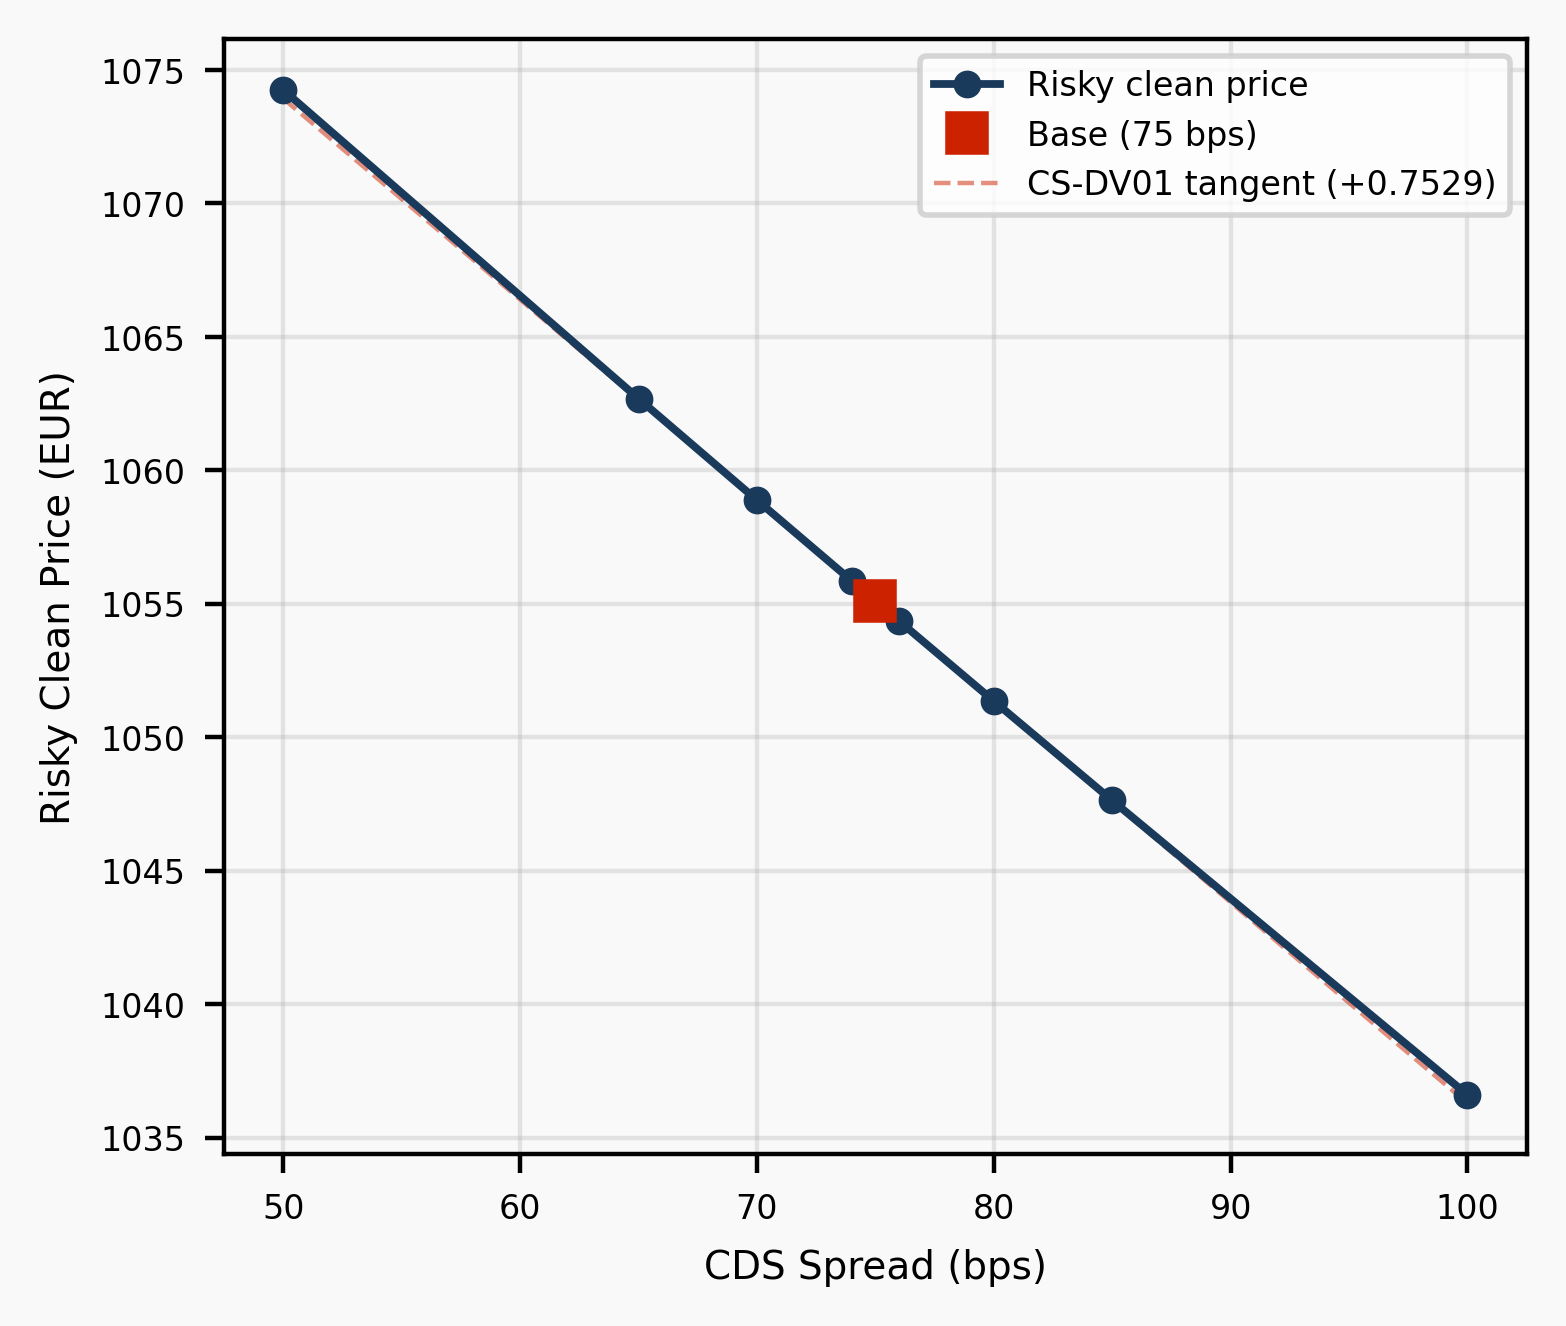
\includegraphics[width=\linewidth]{q15_cs_chart.png}
    \captionof{figure}{Clean price vs.\ CDS spread; dashed line
      shows CS-DV01 tangent at 75~bps.}
    \label{fig:q15_cs}
  \end{minipage}\hfill
  \begin{minipage}[t]{0.46\textwidth}
    \vspace{0pt}
    \centering\scriptsize
    \setlength{\tabcolsep}{2pt}
    \begin{tabular}{@{}rrrrrr@{}}
      \toprule
      \textbf{$\Delta s$} & \textbf{CDS}
        & \textbf{$\Delta$Bnd} & \textbf{MTM}
        & \textbf{$\Delta$Hdg} & \textbf{Red.} \\
      \midrule
      $-$25 &  50 & $+$19.14 & $-$19.02 & $+$0.12 & 99.4\% \\
      $-$10 &  65 & $+$7.58  & $-$7.56  & $+$0.02 & 99.7\% \\
       $-$5 &  70 & $+$3.78  & $-$3.77  & $+$0.00 & 99.9\% \\
       $-$1 &  74 & $+$0.75  & $-$0.75  & $+$0.00 &100\% \\
          0 &  75 &     0.00 &     0.00 &     0.00 &   --- \\
       $+$1 &  76 & $-$0.75  & $+$0.75  & $+$0.00 &100\% \\
       $+$5 &  80 & $-$3.75  & $+$3.76  & $+$0.00 & 99.9\% \\
      $+$10 &  85 & $-$7.48  & $+$7.50  & $+$0.02 & 99.7\% \\
      $+$25 & 100 & $-$18.51 & $+$18.62 & $+$0.12 & 99.4\% \\
      \bottomrule
    \end{tabular}
    \vspace{2pt}
    \captionof{table}{CDS hedge P\&L verification
      (\texteuro{} per 1,000 notional). Avg.\ reduction: 99.7\%.}
    \label{tab:q16_cds_hedge}
  \end{minipage}
\end{figure}

\paragraph{Verification.}
Table~\ref{tab:q16_cds_hedge} shows the hedged portfolio has
near-zero residual P\&L across all bumps, averaging 99.7\% risk
reduction.  The tiny residuals ($\leq$\,\texteuro0.12 at $\pm25$~bps)
come from survival-probability convexity: RPV01 shifts slightly
with the spread level, creating a small second-order mismatch.

\noindent\textbf{Practical limitations.}\quad
(i)~\emph{Maturity mismatch}: the bond matures in 2034 ($\approx$8.6\,yr)
vs.\ a 5Y CDS tenor, so credit DV01 profiles differ.
(ii)~\emph{CDS--bond basis}: CDS and bond credit spreads can
diverge, leaving residual basis risk.
(iii)~\emph{Roll risk}: the 5Y CDS must be rolled at potentially
different spread and RPV01 levels.
(iv)~\emph{Counterparty risk}: we face the CDS seller's credit,
especially in stressed markets.
(v)~\emph{Liquidity}: single-name UniCredit CDS may have wider
bid--offers than iTraxx index CDS.

\subsubsection{Factor Model for Gross Price Changes}
\label{sssec:q17_factor_model}

We combine rate and credit sensitivities into a single linear model:
\begin{equation}
  \Delta GP
  = \alpha
  + \beta_l \,\Delta l
  + \beta_s \,\Delta s
  + \beta_c \,\Delta c
  + \beta_{\text{cds}} \,\Delta\mathit{cds}
  + \varepsilon,
  \label{eq:q17_factor_model}
\end{equation}
where $\Delta l$, $\Delta s$, $\Delta c$ are the monthly PC1--PC3
score changes (bps) and $\Delta\mathit{cds}$ is the CDS spread
change (bps).  We estimate via OLS on 29 joint scenarios that mix
PCA rate shocks ($\pm 0.5\sigma$, $\pm 1\sigma$, $\pm 2\sigma$)
with CDS bumps ($\pm 5$, $\pm 10$, $\pm 25$~bps).

\begin{figure}[htbp]
  \centering
  \begin{minipage}[t]{0.42\textwidth}
    \vspace{0pt}
    \centering\scriptsize
    \setlength{\tabcolsep}{2pt}
    \captionof{table}{OLS four-factor estimates
      (EUR/bps, per \texteuro1,000 notional).}
    \label{tab:q17_factor_model}
    \vspace{2pt}
    \begin{tabular}{@{}lrrr@{}}
      \toprule
      \textbf{Factor} & \textbf{$\hat\beta$}
        & \textbf{SE} & \textbf{$t$} \\
      \midrule
      Intercept ($\alpha$)         & $-$0.50 & 0.376 & $-$1.33 \\
      $\beta_l$ (Level)            & $+$0.110 & 0.011 & $+$10.10 \\
      $\beta_s$ (Slope)            & $-$0.114 & 0.045 & $-$2.54 \\
      $\beta_c$ (Curvature)        & $+$0.044 & 0.123 & $+$0.36 \\
      $\beta_{\text{cds}}$         & $-$0.753 & 0.042 & $-$17.83 \\
      \midrule
      \multicolumn{2}{@{}l}{$R^{2}$ = 0.947} &
      \multicolumn{2}{r}{Adj.\,$R^{2}$ = 0.938} \\
      \multicolumn{2}{@{}l}{RMSE = \texteuro1.84} &
      \multicolumn{2}{r}{$n$ = 29} \\
      \bottomrule
    \end{tabular}
  \end{minipage}\hfill
  \begin{minipage}[t]{0.38\textwidth}
    \vspace{0pt}
    \centering
    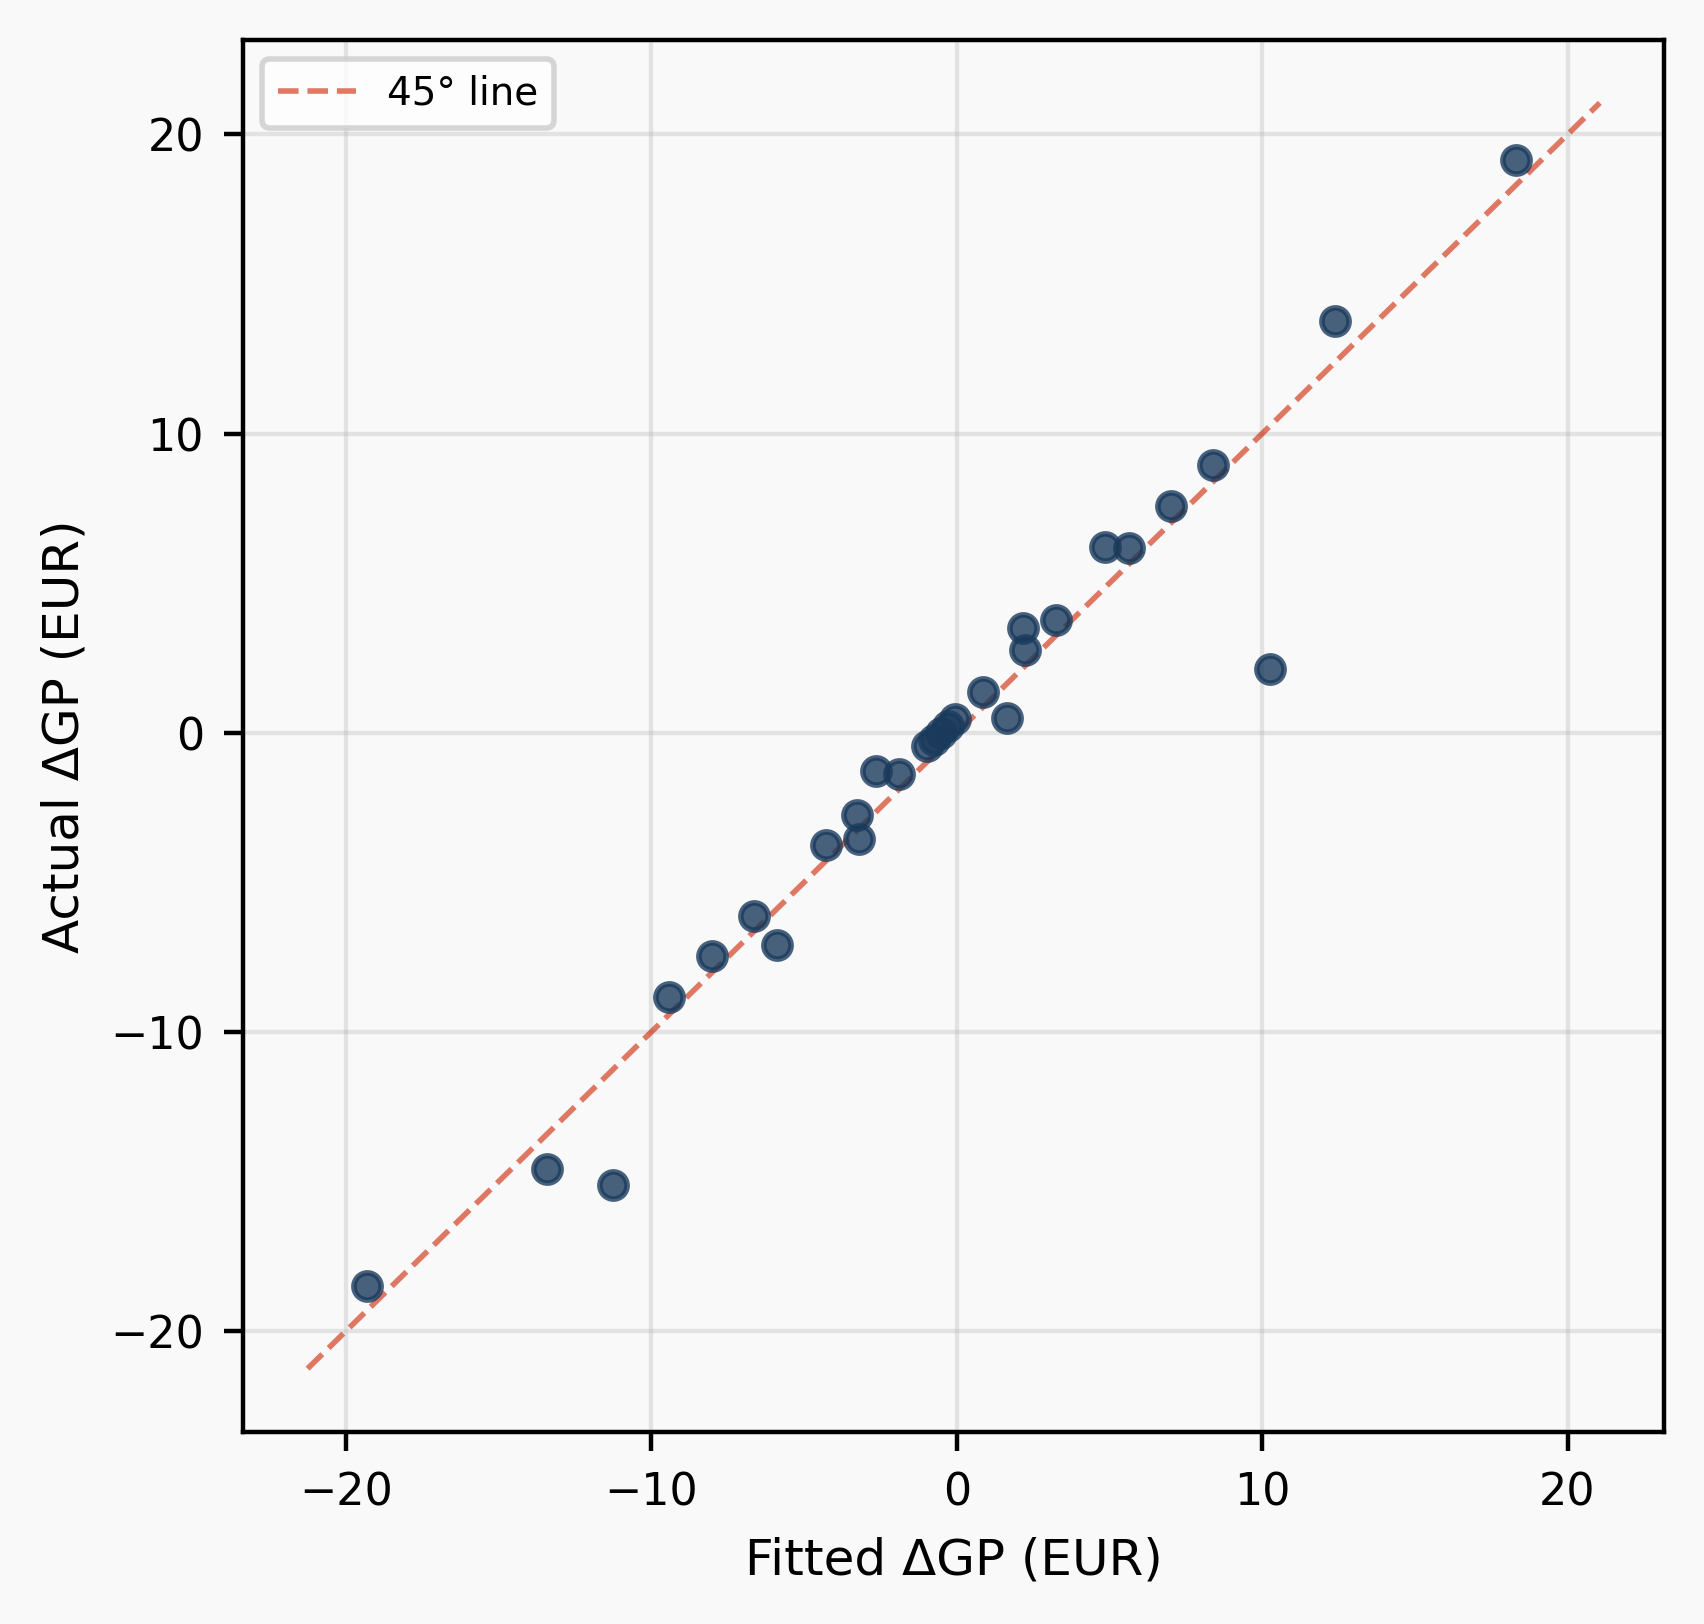
\includegraphics[width=\linewidth]{q17_fitted_vs_actual.png}
    \captionof{figure}{Actual vs.\ fitted $\Delta GP$; deviations
      from the 45\textdegree\ line reflect cap non-linearity.}
    \label{fig:q17_fitted}
  \end{minipage}
\end{figure}

\paragraph{Interpretation.}
The model explains 94.7\% of gross-price variation.  The CDS factor
is the most significant ($t = -17.8$), since CVA moves almost linearly
with spread.  PC1 (level) is the main rate driver ($t = +10.1$), PC2
(slope) is significant at 5\% ($t = -2.5$), and curvature is
insignificant ($t = +0.4$).

\paragraph{Consistency check.}
$\hat\beta_{\text{cds}} = -0.753$~EUR/bp matches the CS-DV01 from
Section~\ref{sssec:q15_cs_dv01}, and $\hat\beta_l$, $\hat\beta_s$ are
consistent with the factor DV01s in Table~\ref{tab:q13_dv01}.

\paragraph{Residual non-linearity.}
The RMSE of \texteuro1.84 (max residual \texteuro8.11) comes mainly from
the PC1 $+2\sigma$ scenario, where the 5.45\% cap creates negative
convexity that a linear model cannot capture.  Excluding the
$\pm 2\sigma$ tail, $R^{2}$ exceeds 99\%.

\subsubsection{Monte Carlo VaR and Expected Shortfall}
\label{sssec:q18_mc_var}

We use the factor model from Section~\ref{sssec:q17_factor_model}
to estimate the 1-month 99\% VaR and ES via Monte Carlo with
$N = 100{,}000$ draws.

We sample each PCA score as $\Delta f_k \sim N(0, \sigma_k^{2})$,
scaling daily eigenvalues to a monthly horizon
($\sigma_k = \sqrt{\lambda_k \times 21}$).  The CDS factor is
$\Delta\mathit{cds} \sim N(0, \sigma_{\text{cds}}^{2})$ with
$\sigma_{\text{cds}} = 3\sqrt{21} \approx 13.7$~bps/month.
All factors are independent, so each simulated P\&L is simply
$\Delta GP_i = \hat\beta_l \Delta l_i + \hat\beta_s \Delta s_i
+ \hat\beta_c \Delta c_i + \hat\beta_{\text{cds}} \Delta\mathit{cds}_i$.

\begin{figure}[htbp]
  \centering
  \begin{minipage}[t]{0.44\textwidth}
    \vspace{0pt}
    \centering\footnotesize
    \setlength{\tabcolsep}{3pt}
    \begin{tabular}{@{}lrrr@{}}
      \toprule
      \textbf{Measure} & \textbf{MC}
        & \textbf{Analyt.} & \textbf{Unit} \\
      \midrule
      Portfolio $\sigma$    & 11.75 & 11.75 & EUR \\
      VaR (99\%)            & 27.34 & 27.32 & EUR \\
      ES  (99\%)            & 31.39 & 31.30 & EUR \\
      VaR \% notional       & 2.73  & 2.73  & \% \\
      ES  \% notional       & 3.14  & 3.13  & \% \\
      \bottomrule
    \end{tabular}
    \vspace{2pt}
    \captionof{table}{1-month 99\% VaR/ES: MC ($N\!=\!100$k)
      vs.\ analytical. Per \texteuro1,000 notional.}
    \label{tab:q18_var}
  \end{minipage}\hfill
  \begin{minipage}[t]{0.52\textwidth}
    \vspace{0pt}
    \centering
    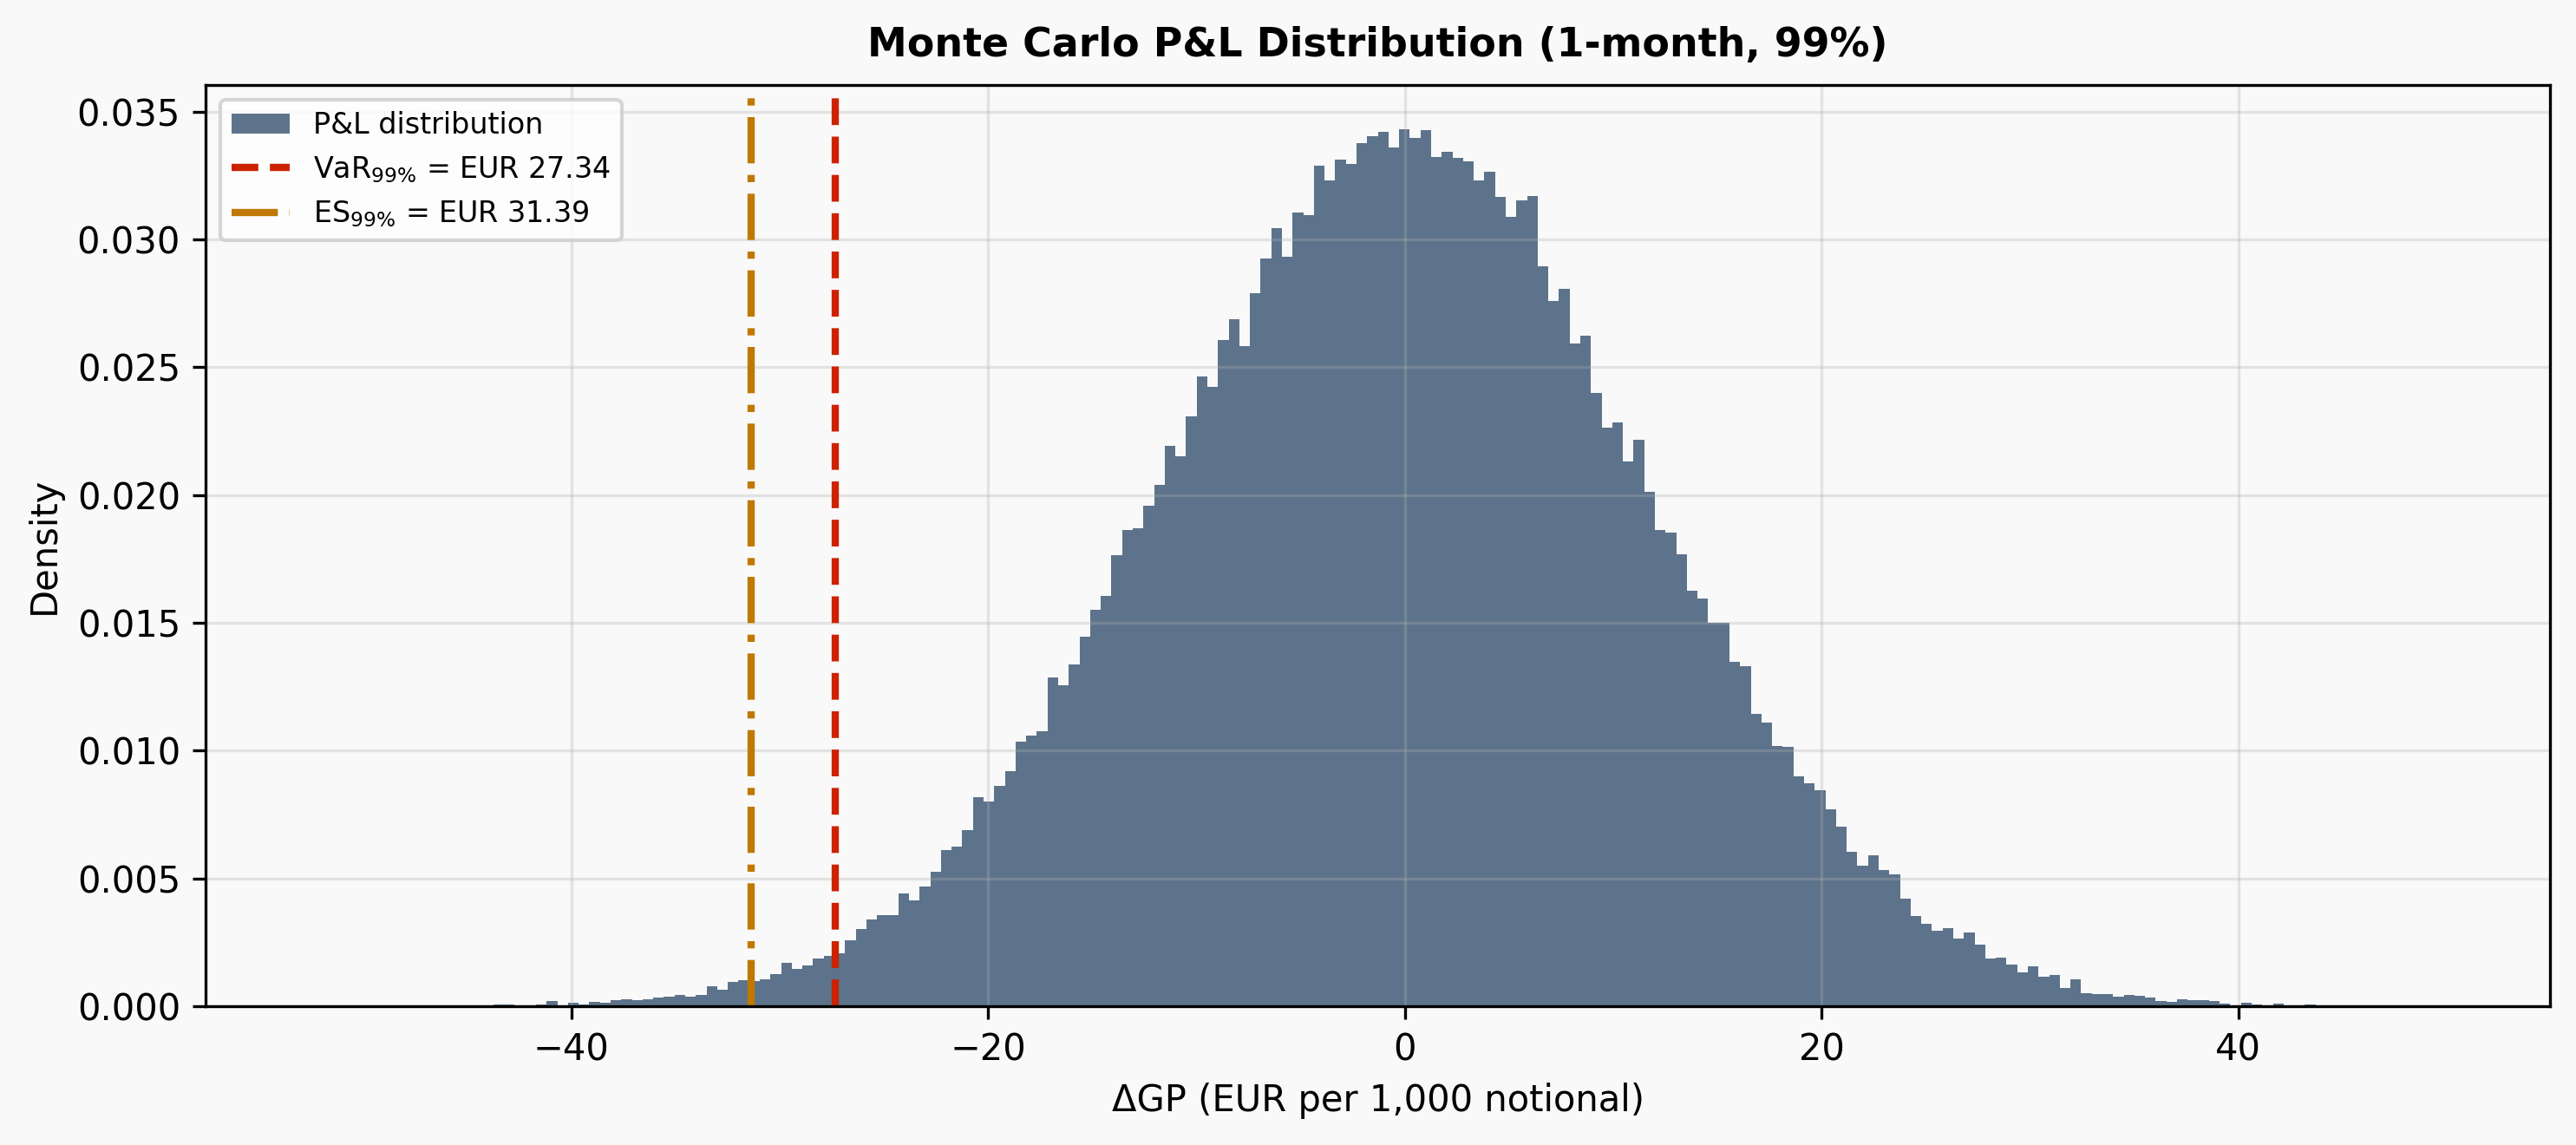
\includegraphics[width=\linewidth]{q18_mc_histogram.png}
    \captionof{figure}{MC P\&L distribution with VaR/ES markers;
      near-zero skew confirms normal assumption.}
    \label{fig:q18_histogram}
  \end{minipage}
\end{figure}

CDS risk dominates the variance (77.7\%), followed by level
(20.9\%), slope (1.4\%) and curvature (0.04\%).  Credit risk
dominates because the bond's long maturity amplifies CVA
sensitivity.  The MC estimates match the analytical benchmarks
closely (VaR ratio 1.0006, ES ratio 1.0026), and the P\&L
distribution is effectively Gaussian---as expected from a
linear-normal model.

\subsubsection{Exact VaR and ES vs.\ Monte Carlo}
\label{sssec:q19_exact}

Since our factor model is linear with independent normal inputs,
the P\&L is itself normal:
\begin{equation}
  \Delta GP \sim N\!\bigl(0,\;\sigma_P^{2}\bigr),
  \qquad
  \sigma_P^{2}
  = \sum_{k} (\beta_k \sigma_k)^{2},
  \label{eq:q19_sigma}
\end{equation}
so we can compute VaR and ES in closed form:
\begin{align}
  \mathrm{VaR}_\alpha &= z_\alpha \,\sigma_P
    = 2.326 \times 11.745
    = \text{\texteuro27.32,}
  \label{eq:q19_var} \\[3pt]
  \mathrm{ES}_\alpha  &= \sigma_P \,
    \frac{\varphi(z_\alpha)}{1-\alpha}
    = 11.745 \times \frac{0.0267}{0.01}
    = \text{\texteuro31.30,}
  \label{eq:q19_es}
\end{align}
where $z_\alpha = \Phi^{-1}(0.99) = 2.3263$.

\begin{figure}[htbp]
  \centering
  \begin{minipage}[t]{0.42\textwidth}
    \vspace{0pt}
    \centering\footnotesize
    \setlength{\tabcolsep}{3pt}
    \begin{tabular}{@{}lrrr@{}}
      \toprule
      \textbf{Measure} & \textbf{Exact}
        & \textbf{MC} & \textbf{Ratio} \\
      \midrule
      $\sigma_P$ (EUR)     & 11.745 & 11.753 & 1.0007 \\
      VaR$_{99\%}$ (EUR)   & 27.32  & 27.34  & 1.0006 \\
      ES$_{99\%}$  (EUR)   & 31.30  & 31.39  & 1.0026 \\
      \bottomrule
    \end{tabular}
    \vspace{2pt}
    \captionof{table}{Exact vs.\ MC risk measures
      (per \texteuro1,000 notional).}
    \label{tab:q19_exact_mc}
  \end{minipage}\hfill
  \begin{minipage}[t]{0.54\textwidth}
    \vspace{0pt}
    \centering
    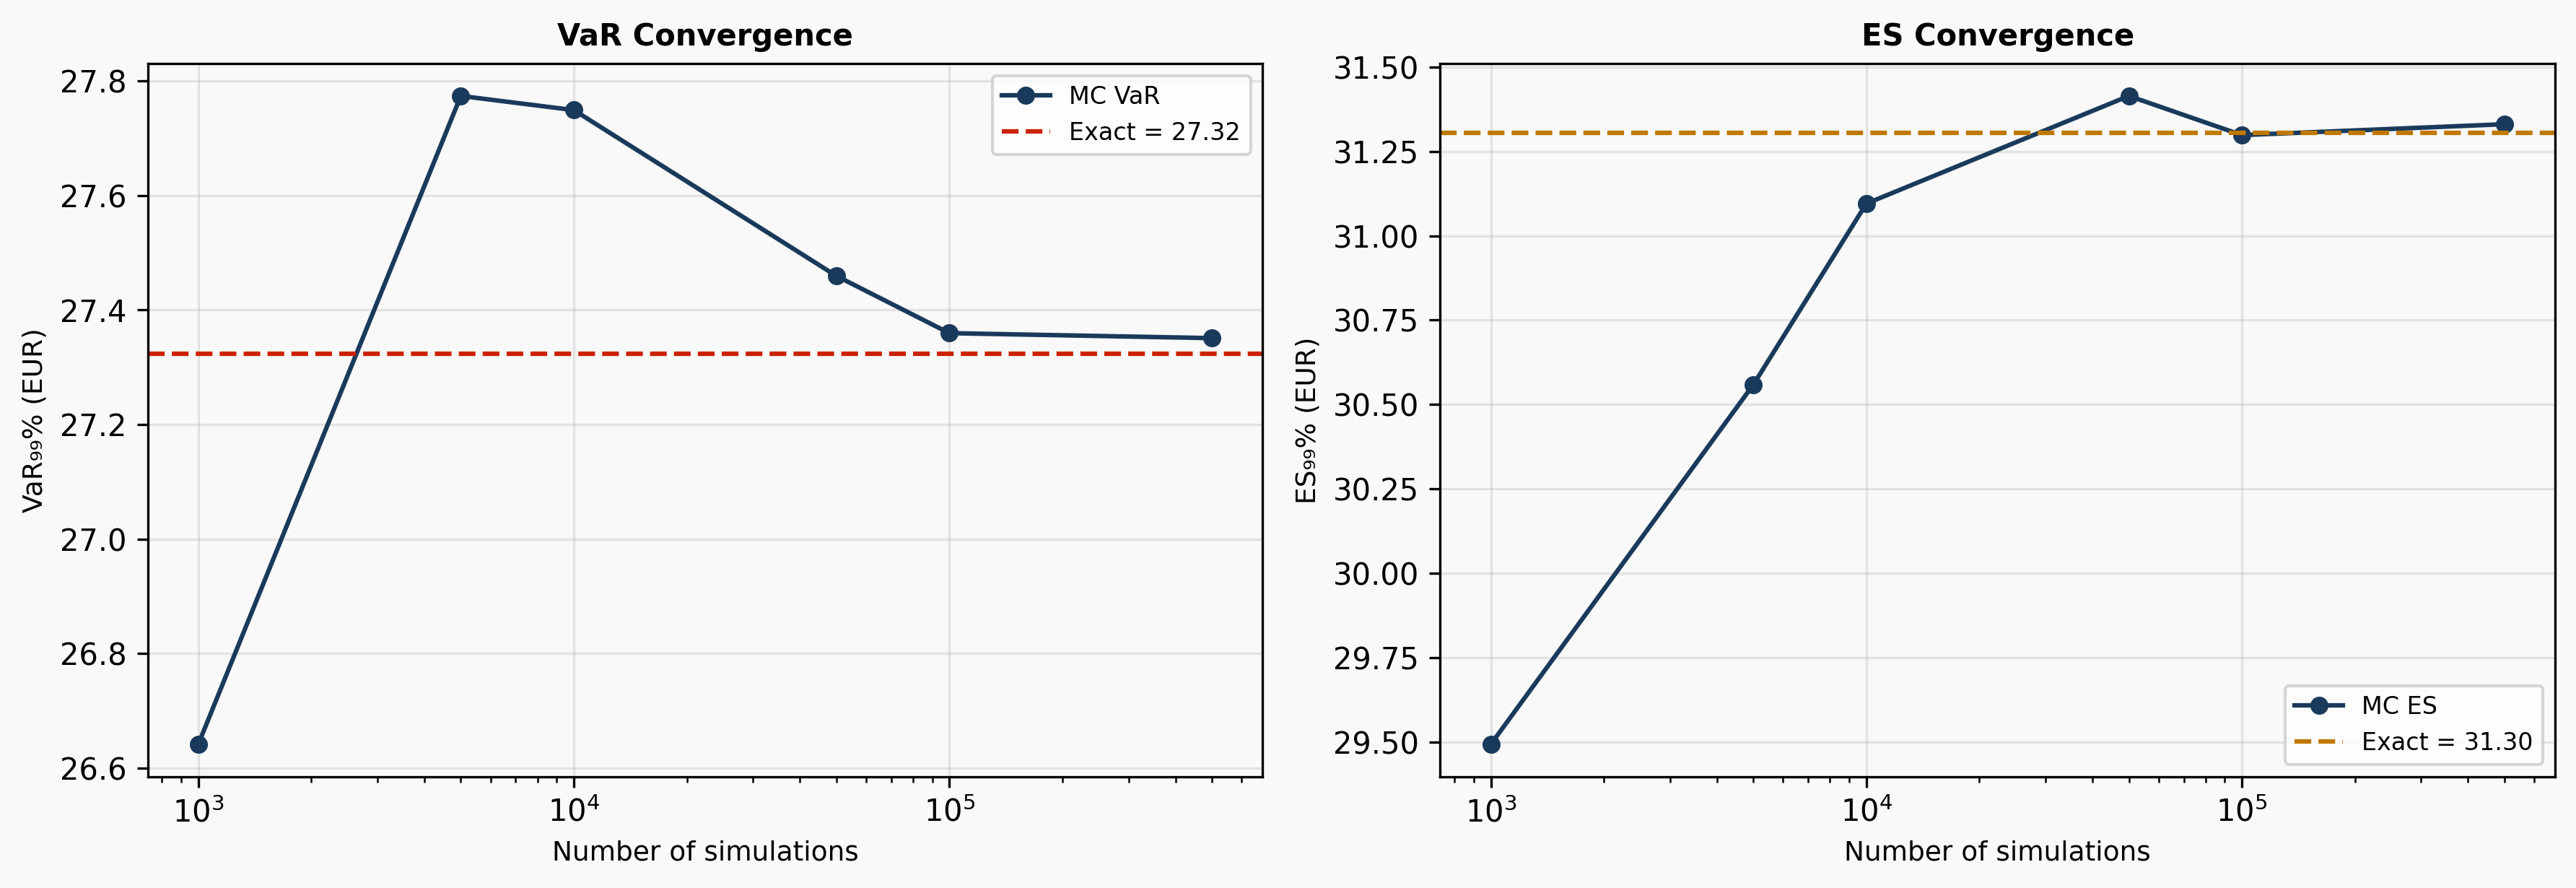
\includegraphics[width=\linewidth]{q19_convergence_chart.png}
    \captionof{figure}{MC VaR/ES convergence to the exact
      normal solution vs.\ number of simulations.}
    \label{fig:q19_convergence}
  \end{minipage}
\end{figure}

Table~\ref{tab:q19_exact_mc} confirms near-perfect agreement
($<$\,0.3\% difference); the residuals are pure sampling noise.
ES converges more slowly because it conditions on the 1\% tail.

The two approaches would diverge if we used
(i)~\emph{non-linear repricing} (capturing the cap's convexity),
(ii)~\emph{fat-tailed factors} (Student-$t$ or jump-diffusion), or
(iii)~\emph{correlated factors} (non-zero credit--rate dependence).

% ------------------------------------------------------------------ Q20
\subsubsection{Marginal and Component VaR Decomposition}
\label{sssec:q20_decomp}

By Euler's theorem, VaR decomposes additively into factor
contributions:
\begin{equation}
  \mathrm{VaR}_\alpha
  = \sum_{k=1}^{4}
  z_\alpha \,\frac{(\beta_k \sigma_k)^2}{\sigma_P}
\end{equation}
where factors are independent so cross-terms vanish.
The marginal VaR measures how total VaR changes per unit
increase in a factor beta:
\begin{equation}
  \mathrm{MVaR}_k
  = z_\alpha \,\frac{\beta_k\,\sigma_k^2}{\sigma_P}
\end{equation}

Table~\ref{tab:q20_decomp} shows that CDS contributes
\texteuro21.22 (77.7\%) of the \texteuro27.32 total VaR,
consistent with Section~\ref{sssec:q18_mc_var}.
Level adds \texteuro5.72 (20.9\%); slope and curvature are
negligible.  The same split applies to ES since the ES
multiplier scales every component equally.

\begin{figure}[htbp]
  \centering
  \begin{minipage}[t]{0.52\textwidth}
    \vspace{0pt}
    \centering\footnotesize
    \setlength{\tabcolsep}{2.5pt}
    \captionof{table}{Component VaR/ES decomposition
      (99\%, 1-month, per \texteuro1,000 notional).}
    \label{tab:q20_decomp}
    \vspace{2pt}
    \begin{tabular}{@{}lrrrrrrr@{}}
      \toprule
      \textbf{Factor} &
      $\beta_k$ &
      $\sigma_k$ &
      $\beta\sigma$ &
      MVaR &
      CVaR &
      CES &
      \% \\
      \midrule
      Level
        & $+$0.110 & 48.89 & $+$5.37
        & $+$52.0 & 5.72 & 6.55 & 20.9 \\
      Slope
        & $-$0.114 & 12.10 & $-$1.38
        & $-$3.3 & 0.38 & 0.43 & 1.4 \\
      Curv.
        & $+$0.044 & 5.19 & $+$0.23
        & $+$0.2 & 0.01 & 0.01 & 0.0 \\
      CDS
        & $-$0.753 & 13.75 & $-$10.35
        & $-$28.2 & 21.22 & 24.31 & 77.7 \\
      \midrule
      \textbf{Total}
        & & & 11.75
        & & \textbf{27.32} & \textbf{31.30} & 100 \\
      \bottomrule
    \end{tabular}
  \end{minipage}\hfill
  \begin{minipage}[t]{0.45\textwidth}
    \vspace{0pt}
    \centering
    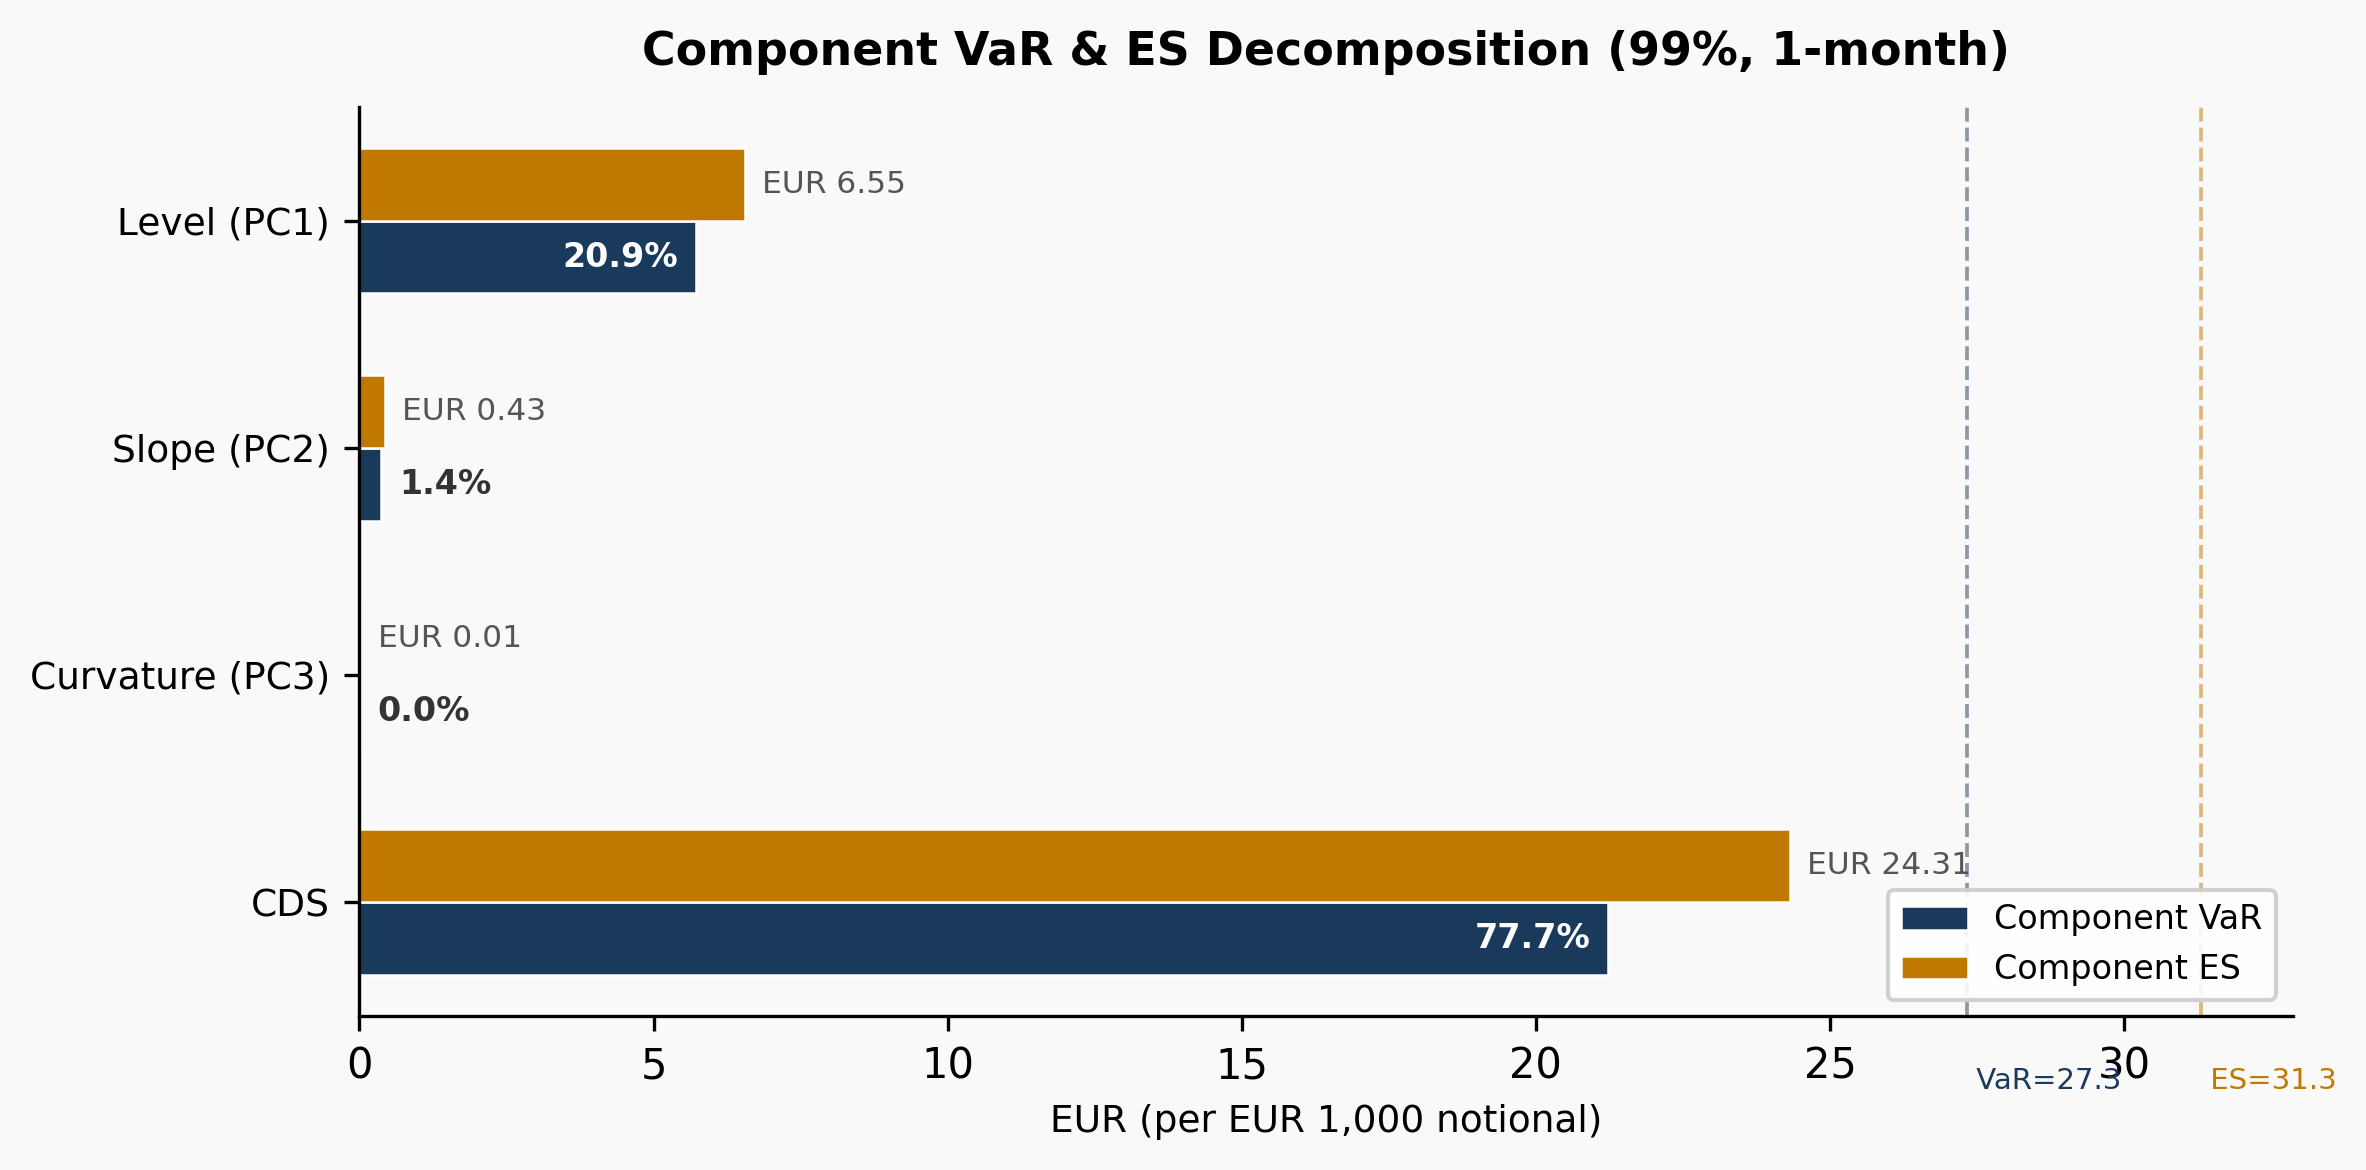
\includegraphics[width=\linewidth]{q20_var_decomposition.png}
    \captionof{figure}{Component VaR/ES by factor; CDS credit
      risk dominates standalone bond risk.}
    \label{fig:q20_decomp}
  \end{minipage}
\end{figure}

The component VaRs sum to \texteuro27.3236 vs.\ the total
of \texteuro27.3235 ($<$\texteuro0.0001 gap), confirming
the exact Euler decomposition.
The CDS factor's marginal VaR of $-28.19$~EUR is the
largest, so the CDS hedge (Section~\ref{sssec:q16_cds_hedge})
gives the biggest single VaR saving.  Combined with the
IRS hedge targeting level risk, the two instruments address
$20.9 + 77.7 = 98.6$\% of standalone risk.

% ------------------------------------------------------------------ Q21
\subsubsection{Hedged-Portfolio VaR Decomposition}
\label{sssec:q21_hedged_var}

We now decompose the VaR of the \textit{fully hedged}
portfolio (bond + IRS hedge from Section~\ref{sssec:q13_hedge}
+ CDS hedge from Section~\ref{sssec:q16_cds_hedge}).
The hedged betas are:
\begin{equation}
  \beta_k^{\,\mathrm{hdg}}
  = \beta_k^{\,\mathrm{bond}}
    + \frac{N_{2\mathrm{Y}}}{10^{6}} \, DV01_k^{2\mathrm{Y}}
    + \frac{N_{10\mathrm{Y}}}{10^{6}} \, DV01_k^{10\mathrm{Y}}
  \qquad (k = 1,2,3)
\end{equation}
and $\beta_{\mathrm{cds}}^{\,\mathrm{hdg}}
= \beta_{\mathrm{cds}}^{\,\mathrm{bond}}
+ \mathrm{RPV01} \times N_{\mathrm{cds}} / 10{,}000$.

Table~\ref{tab:q21_hedged} shows the standalone and hedged VaRs.
The IRS removes slope risk ($\beta_2^{\mathrm{hdg}} \approx 0$)
and the CDS removes credit risk
($\beta_{\mathrm{cds}}^{\mathrm{hdg}} \approx 0$).
Two residuals remain:
(i)~\emph{Level:} the regression beta ($+0.110$) does not match
the DV01 ($+0.144$) used to size the hedge, leaving \texteuro3.68
(88.9\%).
(ii)~\emph{Curvature:} the 10Y swap adds curvature exposure the
hedge does not target, contributing \texteuro0.46 (11.1\%).

\begin{wraptable}{r}{0.50\textwidth}
  \vspace{-10pt}
    \centering\footnotesize
    \setlength{\tabcolsep}{2.5pt}
    \caption{Component VaR: standalone vs.\ hedged
      (99\%, 1-month, per \texteuro1,000 notional).}
    \label{tab:q21_hedged}
    \vspace{2pt}
    \begin{tabular}{@{}lrrrrrr@{}}
      \toprule
      & \multicolumn{3}{c}{Standalone} &
        \multicolumn{3}{c}{Hedged} \\
      \cmidrule(lr){2-4}\cmidrule(lr){5-7}
      Factor &
      $\beta_k$ & CVaR & \% &
      $\beta_k^{\mathrm{h}}$ & CVaR & \% \\
      \midrule
      Level
        & $+$0.110 & 5.72 & 20.9
        & $-$0.034 & 3.68 & 88.9 \\
      Slope
        & $-$0.114 & 0.38 & 1.4
        & $\approx$0 & 0.00 & 0.0 \\
      Curv.
        & $+$0.044 & 0.01 & 0.0
        & $-$0.114 & 0.46 & 11.1 \\
      CDS
        & $-$0.753 & 21.22 & 77.7
        & $\approx$0 & 0.00 & 0.0 \\
      \midrule
      \textbf{Total}
        & & \textbf{27.32} & 100
        & & \textbf{4.15} & 100 \\
      \bottomrule
    \end{tabular}
  \vspace{-8pt}
\end{wraptable}

Overall the hedges cut VaR from \texteuro27.32 to \texteuro4.15
(\textbf{84.8\%}) and ES from \texteuro31.30 to \texteuro4.75.
This linear result \textit{overstates} effectiveness:
Section~\ref{sssec:q14_hedge_impl} showed $-452\%$ hedge
effectiveness at +2$\sigma$ due to the cap's negative convexity.
The true residual VaR would be larger once we include non-linear
repricing, Vega risk, and credit--rate correlation.

% ------------------------------------------------------------------ Q22
\subsubsection{Summary Dashboard}
\label{sssec:q22_summary}

Table~\ref{tab:q22_fv} collects all the main fair-value
and risk results from this analysis.

\begin{table}[htbp]
  \centering\footnotesize
  \setlength{\tabcolsep}{3pt}
  \caption{Summary dashboard (per \texteuro1,000 notional).}
  \label{tab:q22_fv}
  \begin{tabular}{@{}llrl|llrl@{}}
    \toprule
    \multicolumn{4}{c|}{\textit{A. Fair-Value Decomposition}} &
    \multicolumn{4}{c}{\textit{B. Market Comparison}} \\
    \midrule
    & Lev.\ FRN leg & 317.06 & EUR &
    & Mkt clean price & 1,017.00 & EUR \\
    & Net option & $-$28.53 & EUR &
    & Rich/cheap & $+$38.11 & EUR \\
    & Par redemption & 802.26 & EUR &
    & Z-spread (model) & 73.5 & bps \\
    & RF dirty price & \textbf{1,119.32} & EUR &
    & Z-spread (mkt) & 123.0 & bps \\
    & CVA & $-$59.43 & EUR &
    & ASW spread & 132.7 & bps \\
    & Risky dirty & 1,059.89 & EUR &
    & CDS 5Y & 75.0 & bps \\
    & Accrued & $-$4.78 & EUR & & & & \\
    & \textbf{Risky clean} & \textbf{1,055.11} & EUR & & & & \\
    \midrule
    \multicolumn{4}{c|}{\textit{C. Factor Model}} &
    \multicolumn{4}{c}{\textit{D. Hedge Portfolio}} \\
    \midrule
    & $\beta_\ell$ (level) & $+$0.110 & EUR/bp &
    & 2Y IRS (Recv) & 194 & EUR \\
    & $\beta_s$ (slope) & $-$0.114 & EUR/bp &
    & 10Y IRS (Recv) & 429 & EUR \\
    & $\beta_c$ (curv.) & $+$0.044 & EUR/bp &
    & 5Y CDS (Buy) & 1,625 & EUR \\
    & $\beta_{\mathrm{cds}}$ & $-$0.753 & EUR/bp &
    & CDS hedge eff. & 99.7 & \% \\
    & $R^2$ & 94.7 & \% &
    & & & \\
    & CS-DV01 & $+$0.753 & EUR/bp &
    & & & \\
    \midrule
    \multicolumn{4}{c|}{\textit{E. Risk -- Standalone}} &
    \multicolumn{4}{c}{\textit{F. Risk -- Hedged}} \\
    \midrule
    & $\sigma_P$ & 11.75 & EUR &
    & VaR$_{99}$ & \textbf{4.15} & EUR \\
    & VaR$_{99}$ & \textbf{27.32} & EUR &
    & ES$_{99}$ & 4.75 & EUR \\
    & ES$_{99}$ & 31.30 & EUR &
    & VaR reduction & 84.8 & \% \\
    & \;CDS share & 21.22 & (77.7\%) &
    & \;Resid: Level & 3.68 & (88.9\%) \\
    & \;Level share & 5.72 & (20.9\%) &
    & \;Resid: Curv. & 0.46 & (11.1\%) \\
    \bottomrule
  \end{tabular}
\end{table}

Three results stand out.
First, the bond trades \texteuro38 rich to the model because
the market demands a wider spread (123~bps) than the
CDS-implied 75~bps.
Second, credit risk accounts for 77.7\% of standalone VaR,
so the CDS hedge is the single most effective instrument.
Third, the combined IRS+CDS hedge cuts VaR by 84.8\%;
the residual comes from
(i)~the mismatch between regression and DV01 level sensitivities and
(ii)~unhedged curvature from the 10Y swap.

\subsubsection{Comparison with Market Price}
\label{sssec:q10_market}

\needspace{10\baselineskip}
\begin{wraptable}{r}{0.42\textwidth}
  \vspace{-10pt}
  \centering\scriptsize
  \setlength{\tabcolsep}{2pt}
  \begin{tabular}{@{}lrr@{}}
    \toprule
    \textbf{Metric} & \textbf{Val.} & \textbf{Unit} \\
    \midrule
    Model clean       & 105.51 & \% par \\
    Market clean      & 101.70 & \% par \\
    Rich/Cheap        & $+$3.81 & \% par \\
    \midrule
    Z-spr (model)     & $+$73.5 & bps \\
    Z-spr (market)    & $+$123.0 & bps \\
    Z-spr gap         & $-$49.5 & bps \\
    \midrule
    ASW spread        & $+$132.7 & bps \\
    CDS 5Y            & $+$75.0 & bps \\
    CVA-implied       & $+$75.2 & bps \\
    \bottomrule
  \end{tabular}
  \vspace{2pt}
  \caption{Model vs.\ market price
    (5~Nov~2025, EuroTLX mid).}
  \label{tab:q10_comparison}
  \vspace{-8pt}
\end{wraptable}

Table~\ref{tab:q10_comparison} compares our model clean price
(\texteuro1,055.11) with the EuroTLX mid of 101.70\%
(\texteuro1,017.00) on 5~November~2025.\footnote{Source:
Borsa~Italiana EuroTLX for ISIN~IT0005599110;
UniCredit~Bank~GmbH is the sole market maker.}
Our model sits 3.81~pp (\texteuro38.11) above the market,
so the bond looks \emph{rich}.

The market Z-spread (123~bps) is much wider than the 5Y CDS
(75~bps) and our CVA-implied spread (75.2~bps).  We think the
$\approx$48~bps gap comes from:
(i)~\emph{liquidity} ($\approx$30--40~bps)---wide bid--offer
spreads on EuroTLX embed an illiquidity discount
\parencite[Ch.~7]{Tuckman2011};
(ii)~\emph{distribution margin} ($\approx$10--20~bps)---UniCredit
as sole market maker may add a servicing fee;
(iii)~\emph{model simplifications}---flat smile and single curve
may overvalue coupons slightly
(see Section~\ref{sssec:limitations}).

\noindent
Figure~\ref{fig:q10_comparison} shows the rich/cheap analysis:
(a)~price comparison, (b)~Z-spread vs.\ price, (c)~credit spread
decomposition.

\begin{figure}[htbp]
  \centering
  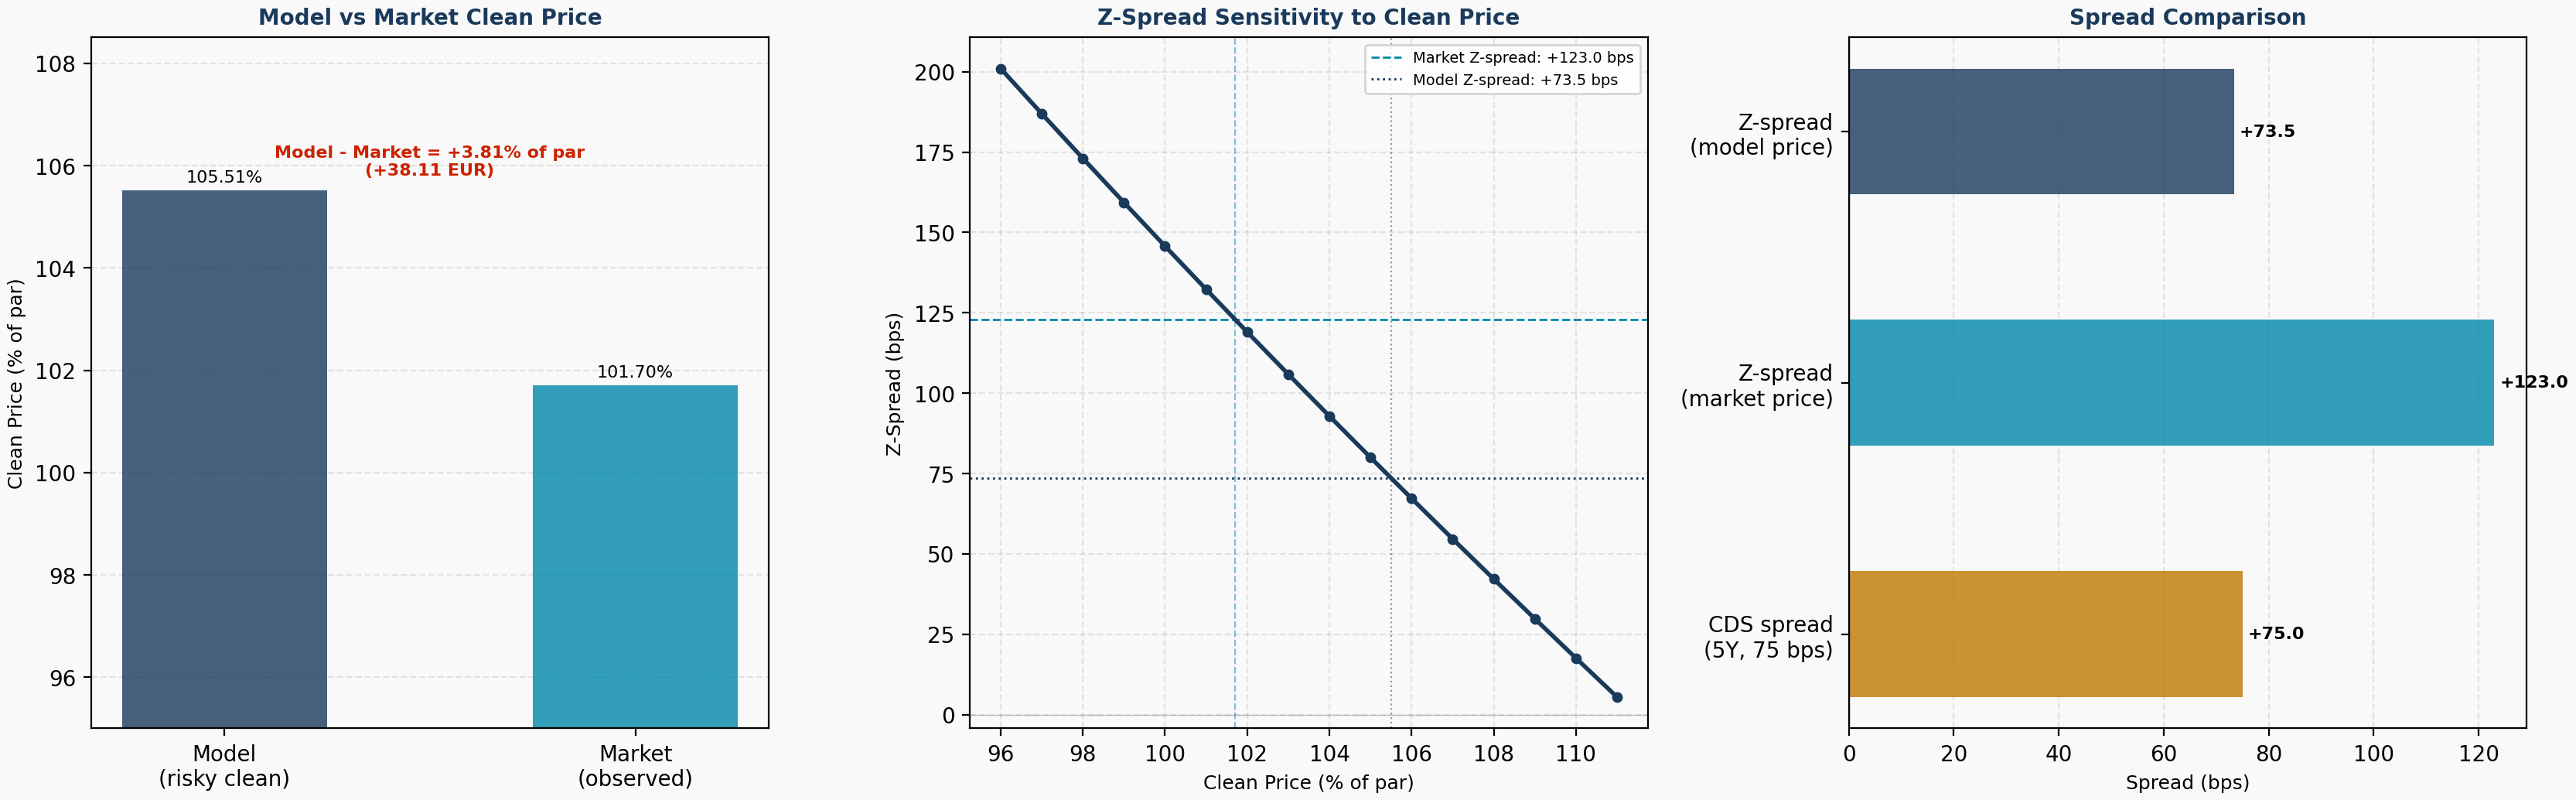
\includegraphics[width=\textwidth]{q10_market_comparison.png}
  \caption{Market comparison: (a)~model vs.\ market price;
    (b)~Z-spread sensitivity; (c)~spread decomposition.}
  \label{fig:q10_comparison}
\end{figure}

\noindent
The ASW spread is 132.7~bps, about 58~bps wider than the CDS
spread.  In liquid markets this basis is typically $\pm$5~bps,
but the wider gap here fits the liquidity and complexity premia
of a retail structured note \parencite[Ch.~12]{Gregory2020}.


\subsection{Discussion}
% Discuss any issues encountered during the analysis.

\subsubsection{Key Findings}

\noindent\textbf{Embedded-option asymmetry.}\quad
We found that the short cap costs roughly ten times the long floor
(\EUR{31.59} vs.\ \EUR{3.06}), so the investor gives away
considerable optionality.  The net option cost of
\EUR{$-28.53$} per \EUR{1\,000} notional cuts fair value
by about 2.85\% versus a plain FRN.

\noindent\textbf{Volatility term structure.}\quad
Stripped Bachelier caplet vols rise from 27.5~bps (1Y) to
73.1~bps (10Y), consistent with the 2025 EUR normal-vol
curve.  This pushes up the cap cost for later coupons.

\noindent\textbf{CVA and credit risk.}\quad
The CVA of \EUR{59.43} (5.94\% of notional) is the
second-largest adjustment.  Together with the net option cost,
they reduce value by $\approx$8.8\% of notional versus a
risk-free FRN.  A BBB$-$ issuer at 200~bps CDS would roughly
triple the CVA.


\subsubsection{Issues and Limitations Encountered}
\label{sssec:limitations}

\noindent\textbf{Cap non-linearity.}\quad
The capped coupon creates strong negative convexity.
Our linear model fits well ($R^2=94.7\%$) but residuals
reach \texteuro8.1 at +2$\sigma$, and the IRS hedge shows
$-452\%$ effectiveness there
(Section~\ref{sssec:q14_hedge_impl}).  Full QuantLib
repricing would be needed in practice.

\noindent\textbf{Single-curve framework.}\quad
We use one curve for discounting and projection, which
overstates long-maturity discount factors by 5--10~bps
(OIS--Euribor basis), biasing the price upward.

\noindent\textbf{Credit--rate independence.}\quad
We treat CDS and rate factors as independent; in a
stress event they would co-move, weakening the hedge.

\noindent\textbf{Constant hazard rate.}\quad
Our CVA uses a flat hazard rate from the 5Y CDS;
a piecewise calibration would be more accurate.

\noindent\textbf{CDS vol assumption.}\quad
We use 3~bps/day (typical IG); actual vol may be higher
in stress, underestimating tail risk.

% ────────────────────────────────────────────────────────────────────────────
\section{Conclusions}
% Summarize the key findings and conclusions drawn from the analysis.

We priced and analysed a UniCredit variable-rate bond
(ISIN IT0005599110) with a 1.60$\times$ Euribor~3M coupon,
capped at 5.45\% and floored at 0\%.

\noindent\textbf{Fair value.}\quad
We decomposed the bond into a leveraged FRN leg (EUR\,317),
a net option component (EUR\,$-29$), and par redemption
(EUR\,802), giving a risk-free dirty price of EUR\,1,119.
After a CVA of EUR\,59 (75~bps CDS, 40\% recovery),
the credit-adjusted clean price is
\textbf{EUR\,1,055.11}.  The market quotes EUR\,1,017,
a EUR\,38 gap driven by the wider market Z-spread
(123~bps) versus the CDS-implied 75~bps.

\noindent\textbf{Risk profile.}\quad
Our four-factor model captures 94.7\% of price variation.
The 99\% 1-month VaR is EUR\,27.32 (CDS: 77.7\%,
level: 20.9\%).  ES is EUR\,31.30.

\noindent\textbf{Hedging.}\quad
A 2Y\,+\,10Y IRS hedge (EUR\,194 and EUR\,429) plus a
5Y CDS position (EUR\,1,625) cuts VaR by 84.8\% to
EUR\,4.15.  The residual comes from unhedged curvature
and a beta--DV01 mismatch on the level factor.

\noindent\textbf{Caveats.}\quad
The linear model overstates hedge effectiveness:
full repricing at +2$\sigma$ showed $-452\%$ due to
the cap's negative convexity.  A production framework
should use full MC repricing, allow credit--rate
correlation, and add Vega hedges.

\newpage
\section{Bibliography}
\printbibliography[heading=none]



\newpage
\appendix
\section{List of Acronyms}
\label{sec:acronyms}

\begin{table}[H]
\centering
\small
\begin{tabular}{@{}ll@{}}
\toprule
\textbf{Acronym} & \textbf{Definition} \\
\midrule
AB6E      & Annual Basis 6-month EURIBOR (Refinitiv ticker convention) \\
ACT/360   & Actual/360 day count convention \\
ASW       & Asset Swap (spread) \\
ATM       & At The Money \\
CCP       & Central Counterparty Clearing \\
CDS       & Credit Default Swap \\
CIR       & Cox--Ingersoll--Ross (interest rate model) \\
CS-DV01   & Credit Spread DV01 \\
CVA       & Credit Valuation Adjustment \\
DF        & Discount Factor \\
DV01      & Dollar Value of 01 (price change per 1 basis point) \\
ECB       & European Central Bank \\
EE        & Expected Exposure \\
EMTN      & Euro Medium Term Note \\
ES        & Expected Shortfall \\
EURIBOR   & Euro Interbank Offered Rate \\
FRN       & Floating Rate Note \\
IRS       & Interest Rate Swap \\
ISIN      & International Securities Identification Number \\
LSEG      & London Stock Exchange Group \\
MC        & Monte Carlo \\
MFBD      & Modified Following Business Day \\
MOT       & Mercato Obbligazionario Telematico \\
MREL      & Minimum Requirement for own funds and Eligible Liabilities \\
NPV       & Net Present Value \\
OIS       & Overnight Index Swap \\
OLS       & Ordinary Least Squares \\
O/N       & Overnight (deposit rate) \\
P\&L      & Profit and Loss \\
PC        & Principal Component \\
PCA       & Principal Component Analysis \\
PV        & Present Value \\
RMSE      & Root Mean Square Error \\
RPV01     & Risky PV01 (present value of 1 basis point) \\
TARGET    & Trans-European Automated Real-time Gross Settlement Express Transfer \\
VaR       & Value at Risk \\
Z-spread  & Zero-volatility spread \\
\bottomrule
\end{tabular}
\caption{Acronyms and abbreviations used in this report.}
\label{tab:acronyms}
\end{table}

% ────────────────────────────────────────────────────────────────────────────
\newpage
\section{Reproduction Guide}
\label{sec:repro}

All source code is hosted on GitHub.  Follow the steps below to
replicate every result, table, and chart.

\paragraph{Environment Setup.}

\begin{enumerate}[leftmargin=*]\setlength{\itemsep}{2pt}
  \item \textbf{Clone the repository:}
\begin{verbatim}
git clone https://github.com/manpreet-sangha/SMM269_Fixed_Income.git
cd SMM269_Fixed_Income
\end{verbatim}

  \item \textbf{Create and activate a virtual environment:}

  \textit{Windows:}
\begin{verbatim}
python -m venv .venv
.venv\Scripts\activate
\end{verbatim}

  \textit{macOS / Linux:}
\begin{verbatim}
python3 -m venv .venv
source .venv/bin/activate
\end{verbatim}

  \item \textbf{Install all dependencies:}
\begin{verbatim}
pip install -r requirements.txt
\end{verbatim}
\end{enumerate}

\paragraph{Running the Scripts.}

\begin{enumerate}[leftmargin=*]\setlength{\itemsep}{2pt}
  \item \textbf{Run the pricing scripts} in order.  Each question folder
    is self-contained; outputs are written to its \texttt{output/}
    sub-directory.


\end{document}
